% !TEX program = xelatex
% ============================================================
%  Магистерская диссертация — AgentsSwarm
%  Компилировать: xelatex ВКР.tex  (дважды для TOC)
%  ТРЕБОВАНИЕ: Конвертируйте Титульный_лист.docx → Титульный_лист.pdf
%              и положите рядом с этим файлом перед компиляцией.
% ============================================================
\documentclass[14pt,a4paper]{extreport}

% ---------- Кодировка и язык ----------
\usepackage{fontspec}
\usepackage[main=russian,english]{babel}
\setmainfont{Times New Roman}
\setsansfont{Arial}
\setmonofont[Scale=0.85]{Courier New}

% \Asbuk для приложений (А, Б, В ...) — если babel-russian не определяет
\providecommand{\Asbuk}[1]{%
  \ifcase\value{#1}\or А\or Б\or В\or Г\or Д\or Е\or Ж\or З\or И\or К%
  \or Л\or М\or Н\or О\or П\or Р\or С\or Т\or У\or Ф\fi
}

% ---------- Поля ----------
\usepackage[
  left=30mm,
  right=15mm,
  top=20mm,
  bottom=20mm,
  headheight=14pt
]{geometry}

% ---------- Межстрочный интервал и абзац ----------
\usepackage{setspace}
\onehalfspacing
\usepackage{indentfirst}
\setlength{\parindent}{1.25cm}

% ---------- Заголовки ----------
\usepackage{titlesec}

\titleformat{\chapter}[block]
  {\centering\bfseries\large}
  {ГЛАВА~\thechapter.\quad}
  {0pt}
  {}
\titlespacing*{\chapter}{0pt}{0pt}{24pt}

% Ненумерованные главы (Введение, Заключение)
\titleformat{name=\chapter,numberless}[block]
  {\centering\bfseries\large}
  {}
  {0pt}
  {}
\titlespacing*{name=\chapter,numberless}{0pt}{0pt}{24pt}

\titleformat{\section}[block]
  {\bfseries\normalsize}
  {\thesection.\quad}
  {0pt}
  {}
\titlespacing*{\section}{0pt}{14pt}{6pt}

\titleformat{\subsection}[block]
  {\bfseries\normalsize}
  {\thesubsection.\quad}
  {0pt}
  {}
\titlespacing*{\subsection}{0pt}{10pt}{4pt}

\titleformat{\subsubsection}[block]
  {\bfseries\normalsize}
  {\thesubsubsection.\quad}
  {0pt}
  {}
\titlespacing*{\subsubsection}{0pt}{8pt}{4pt}

% ---------- Нумерация страниц ----------
% plain: номер по центру снизу — стандарт для российских ВКР
\pagestyle{plain}

% ---------- Графика ----------
\usepackage{graphicx}
\graphicspath{{./img/}}
\usepackage{float}
\usepackage{pdflscape}

% ---------- Подписи ----------
\usepackage{caption}
\captionsetup[figure]{
  justification=centering,
  labelsep=period,
  name=Рис.,
  font=small
}
\captionsetup[table]{
  justification=raggedright,
  singlelinecheck=false,
  labelsep=period,
  name=Таблица,
  font=small
}

% ---------- Таблицы ----------
\usepackage{booktabs}
\usepackage{array}
\usepackage{longtable}
\usepackage{multirow}

% ---------- Математика ----------
\usepackage{amsmath,amssymb}

% ---------- Листинги ----------
\usepackage{listings}
\usepackage{xcolor}
\definecolor{codegray}{rgb}{0.5,0.5,0.5}
\definecolor{codeblue}{rgb}{0.1,0.1,0.9}
\definecolor{backcolour}{rgb}{0.96,0.96,0.94}
\lstdefinestyle{mystyle}{
  backgroundcolor=\color{backcolour},
  commentstyle=\color{codegray},
  keywordstyle=\color{codeblue},
  basicstyle=\ttfamily\small,
  breaklines=true,
  keepspaces=true,
  numbers=left,
  numberstyle=\tiny\color{codegray},
  numbersep=5pt,
  showstringspaces=false,
  tabsize=2
}
\lstset{style=mystyle}

% ---------- Гиперссылки ----------
\usepackage{hyperref}
\hypersetup{
  colorlinks=true,
  linkcolor=black,
  citecolor=black,
  urlcolor=blue,
  bookmarksnumbered=true,
  pdftitle={Организация кооперативного восприятия сцены в группе автономных агентов},
  pdfauthor={}
}

% ---------- Титульный лист (PDF) ----------
\usepackage{pdfpages}

% ---------- Улучшенные таблицы ----------
\usepackage{array}

% ---------- Списки ----------
\usepackage{enumitem}
\setlist{noitemsep, topsep=4pt, leftmargin=1.25cm}

% ---------- Нумерация рисунков и таблиц по главам ----------
% \counterwithin встроен в LaTeX2e >= 2018, chngcntr не нужен
\counterwithin{figure}{chapter}
\counterwithin{table}{chapter}
\counterwithin{equation}{chapter}

% ---------- Оглавление ----------
\usepackage{tocloft}
% Babel сбрасывает \contentsname при загрузке — переопределяем через addto
\addto\captionsrussian{\renewcommand{\contentsname}{СОДЕРЖАНИЕ}}
\addto\captionsrussian{\renewcommand{\chaptername}{Глава}}
\renewcommand{\cftchapfont}{\bfseries}
\renewcommand{\cftchappagefont}{\bfseries}
\renewcommand{\cftchapleader}{\cftdotfill{\cftdotsep}}
\setlength{\cftbeforechapskip}{4pt}

% ---------- Приложения ----------
% appendix.sty не требуется — используем стандартный \appendix

% ---------- Переносы и переполнение строк ----------
% hyphens передаём url ДО загрузки hyperref (который его подгружает)
\PassOptionsToPackage{hyphens}{url}
\tolerance=1500
\emergencystretch=2em

% ============================================================
\begin{document}
\pagenumbering{arabic}
\setcounter{page}{1}

% ============================================================
%  ТИТУЛЬНЫЙ ЛИСТ
% ============================================================
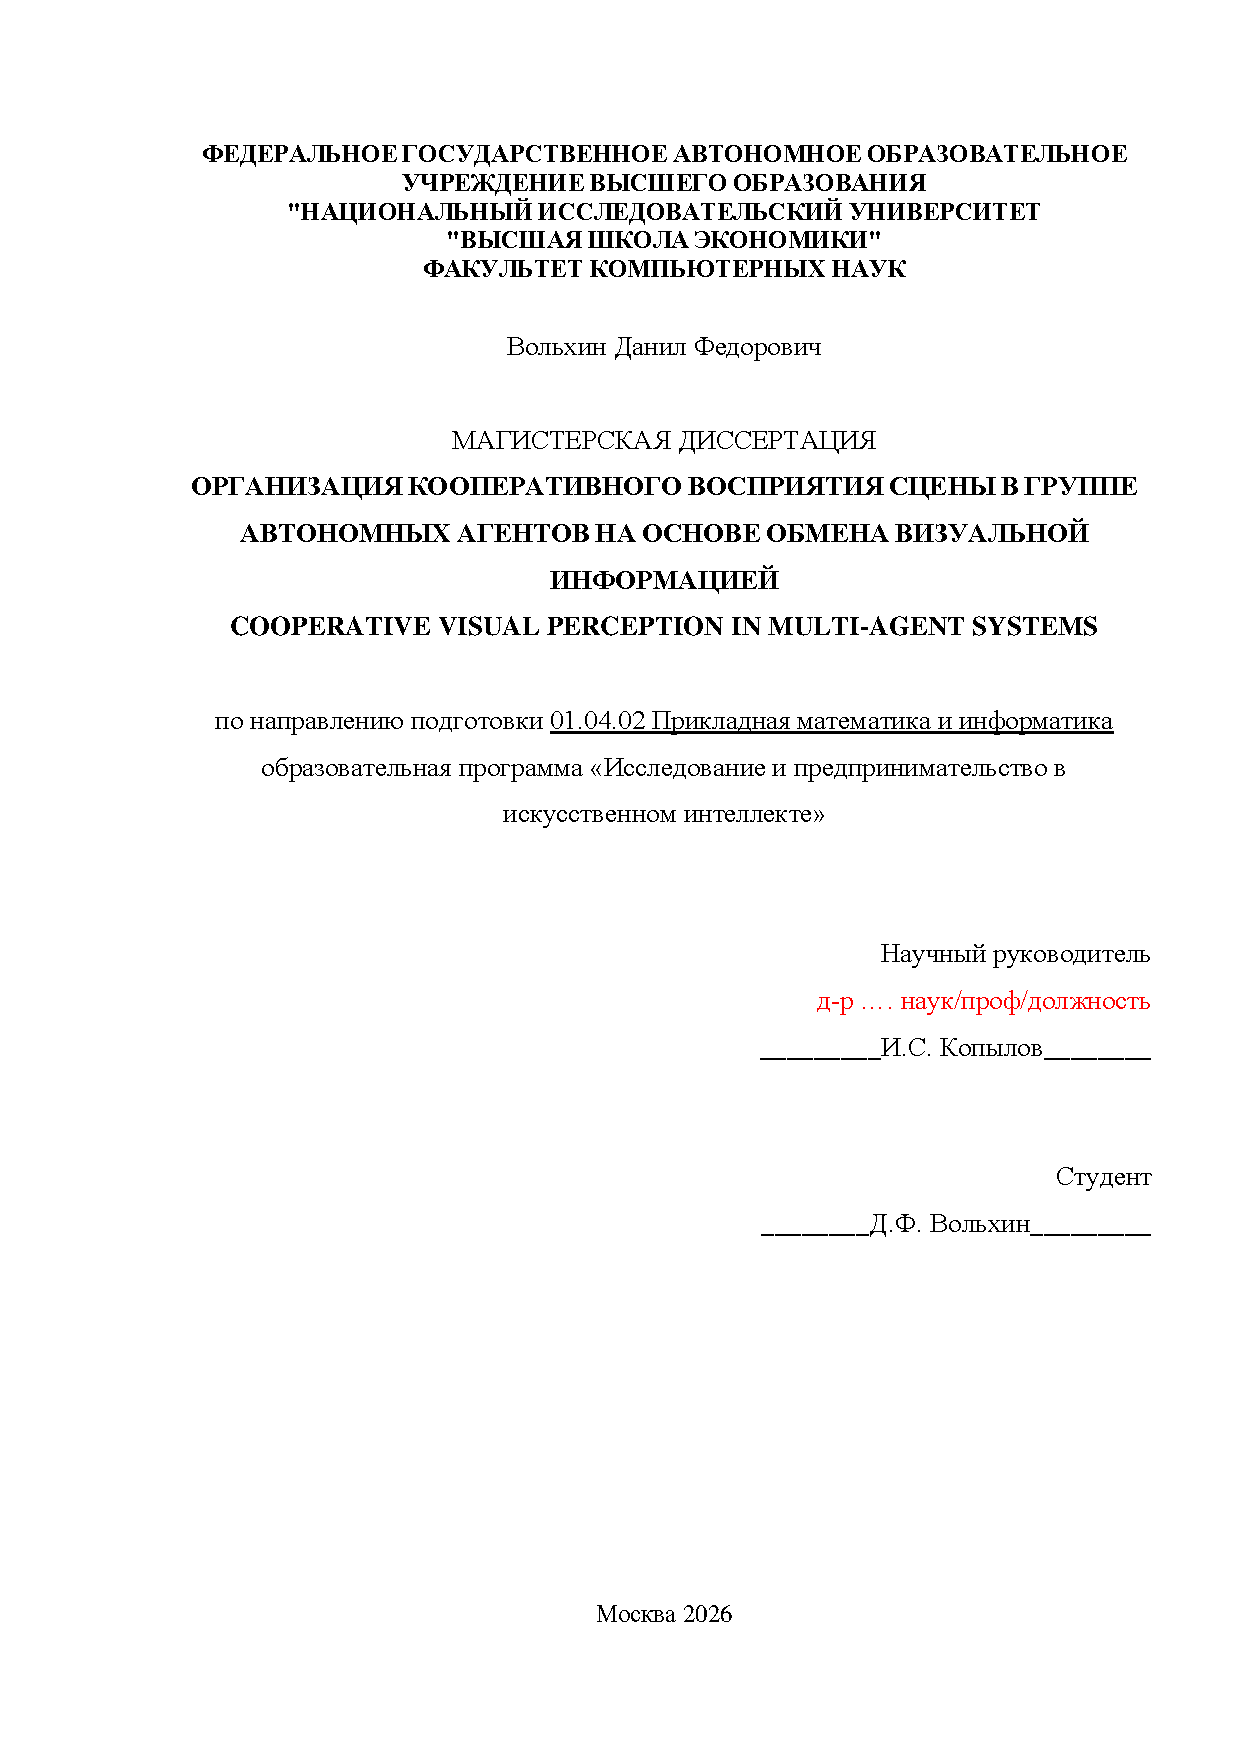
\includepdf[pages=-]{Титульный_лист_flat.pdf}

% ============================================================
%  АННОТАЦИЯ НА РУССКОМ
% ============================================================
\newpage
\thispagestyle{empty}
\begin{center}
  \textbf{АННОТАЦИЯ}
\end{center}
\medskip

Работа посвящена проектированию и реализации многоагентной робототехнической платформы AgentsSwarm, обеспечивающей кооперативное восприятие сцены группой мобильных роботов, стандартизованное управление флотом и высокоуровневую оркестрацию задач посредством больших языковых моделей.

\textbf{Цель работы}~--- создание интегрированного программного комплекса, в котором запрос пользователя на естественном языке транслируется в скоординированное выполнение миссий группой роботов через единый сквозной контур управления.

\textbf{Задачи:} анализ подходов к кооперативному восприятию и координации многороботных систем; разработка микросервисной архитектуры из восьми взаимосвязанных компонентов; реализация LLM"=оркестратора на базе OpenAI Agents SDK с маршрутизатором Router, планировщиком, исполнителем PlanRunner и агентами RobotInfo, MapAnalyst, Navigation, SwarmCoordinator и General; переработка трёх MCP"=серверов (Mission Control, Mission Dispatch, ros-msp) с переходом на асинхронную модель вызовов; адаптация форков NVIDIA Mission Control и Mission Dispatch под протокол VDA5050; экспериментальная оптимизация VLA"=модели SmolVLA для бортового инференса.

\textbf{Методология} основана на принципах облачной робототехники, событийно"=ориентированной архитектуры и протокола Model Context Protocol. Эмпирическая база включает симуляцию флота роботов Carter в NVIDIA Isaac Sim (headless"=режим, ROS~2 Jazzy, rosbridge WebSocket); развёртывание LLM"=сервиса Qwen2.5"=Instruct в режиме Data Parallel на двух узлах Tesla V100 (32~ГБ VRAM) через авторский vLLM"=сервис; пайплайн дистилляции, прунинга и квантизации модели SmolVLA.

\textbf{Результаты:} реализованы восемь самостоятельных компонентов~--- Interface (React + FastAPI + Celery, 168~коммитов, срез v0.5.0), Orchestrator (FastAPI + Agents SDK, 61~коммит, срез v0.5.6), vLLM Service (Data Parallel, срез v0.2.9), доработанные форки Mission Control и Mission Dispatch, настроенный ROS~2 workspace, три переработанных MCP"=сервера. Контрольный локальный pytest-прогон актуального кода Orchestrator подтвердил 66 из 88 тестов; оставшиеся падения связаны с рассинхронизацией тестовых ожиданий после изменения PlanRunner/MapAnalyst и с проверками LLM-клиента. Для модели SmolVLA достигнуто сжатие в 443 раза по числу параметров при сохранении более 90\% точности (MSE~+9{,}1\%, $R^2$~$-$1{,}8\%) и ускорении инференса в 25~раз (450~мс~$\to$~18~мс, RTX~4090).

% ============================================================
%  ABSTRACT (EN)
% ============================================================
\newpage
\thispagestyle{empty}
\begin{center}
  \textbf{ABSTRACT}
\end{center}
\medskip

This thesis presents the design and implementation of AgentsSwarm, a multi"=agent robotic platform that enables cooperative scene perception among a group of mobile robots, standardised fleet management, and high"=level task orchestration driven by large language models.

\textbf{The objective} is to build an integrated software system in which a natural"=language user request is translated into coordinated multi"=robot mission execution through a unified end"=to"=end control pipeline.

\textbf{Research tasks:} analysis of cooperative perception and multi"=robot coordination approaches; design of a microservice architecture comprising eight interconnected components; development of an LLM orchestrator based on the OpenAI Agents SDK with Router, a planner, PlanRunner, and the RobotInfo, MapAnalyst, Navigation, SwarmCoordinator, and General agents; rework of three MCP servers (Mission Control, Mission Dispatch, ros-msp) with a migration to asynchronous tool calls; adaptation of NVIDIA Mission Control and Mission Dispatch forks to the VDA5050 protocol; and experimental optimisation of the SmolVLA vision"=language"=action model for on"=board inference.

\textbf{The methodology} is grounded in cloud"=robotics principles, event"=driven architecture, and the Model Context Protocol. The empirical base comprises simulation of a Carter robot fleet in NVIDIA Isaac Sim (headless mode, ROS~2 Jazzy, rosbridge WebSocket); deployment of a Qwen2.5"=Instruct LLM service in Data Parallel mode across two Tesla V100 nodes (32~GB VRAM each) via a custom"=built vLLM service; and a knowledge"=distillation, pruning, and quantisation pipeline for SmolVLA.

\textbf{Results:} eight independent components were implemented~--- Interface (React + FastAPI + Celery, 168~commits, v0.5.0 development snapshot), Orchestrator (FastAPI + Agents SDK, 61~commits, v0.5.6 development snapshot), vLLM Service (Data Parallel, v0.2.9 development snapshot), reworked Mission Control and Mission Dispatch forks, a configured ROS~2 workspace, and three redesigned MCP servers. A local pytest control run of the current Orchestrator code passed 66 of 88 tests; the remaining failures are related to outdated test expectations after PlanRunner/MapAnalyst changes and LLM-client checks. The SmolVLA model was compressed 443"=fold in parameter count while retaining over 90\% accuracy (MSE~+9.1\%, $R^2$~$-$1.8\%) with a 25$\times$ inference speed"=up (450~ms~$\to$~18~ms on RTX~4090).

% ============================================================
%  ОГЛАВЛЕНИЕ
% ============================================================
\newpage
\tableofcontents

% ============================================================
%  ВВЕДЕНИЕ
% ============================================================
\chapter*{ВВЕДЕНИЕ}
\addcontentsline{toc}{chapter}{ВВЕДЕНИЕ}

Современная промышленная робототехника переживает качественный переход от использования одиночных роботов-исполнителей к развёртыванию гетерогенных флотов автономных мобильных роботов (AMR) и автоматизированных транспортных средств (AGV). Задачи складской логистики, промышленной инспекции, гибкого производства всё чаще требуют координированного взаимодействия группы роботов, способных воспринимать и интерпретировать общее пространство операций. Одиночный агент принципиально ограничен угловым полем зрения, дальностью сенсоров и локальными вычислительными ресурсами; группа же агентов, обменивающихся перцептивной информацией, способна совместно формировать наблюдение сцены, недоступное ни одному из них в отдельности.

Вместе с тем координация флота остаётся нетривиальной инженерной задачей. Существующие fleet management системы~--- в том числе соответствующие стандарту VDA5050~--- предоставляют надёжный низкоуровневый контур диспетчеризации миссий, однако не обеспечивают высокоуровневого семантического планирования и не предоставляют пользователю интерфейс на естественном языке. Академические прототипы кооперативного восприятия (V2VNet, Where2comm, CoBEVT) достигают высоких показателей точности на симулированных датасетах, однако не интегрированы с промышленными стандартами координации флота.

Появление мощных больших языковых моделей (LLM) открывает возможность транслировать пользовательский запрос на естественном языке напрямую в координированное выполнение многороботных миссий. Парадигмы ReAct и вызова инструментов превращают языковую модель из диалогового интерфейса в рассуждающего агента, способного обращаться к внешним сервисам, накапливать наблюдения и корректировать план действий.

\textbf{Объект исследования}~--- многоагентная робототехническая система с кооперативным восприятием и централизованным fleet management.

\textbf{Предмет исследования}~--- методы организации взаимодействия, координации и LLM-планирования в группе автономных агентов.

\textbf{Методы исследования:} системный анализ, микросервисное проектирование, симуляционный эксперимент, дистилляция нейронных сетей.

\textbf{Цель работы}~--- создание интегрированного программного комплекса AgentsSwarm, в котором запрос пользователя на естественном языке транслируется в скоординированное выполнение миссий группой роботов через единый сквозной контур управления.

Для достижения цели решены следующие \textbf{задачи}:
\begin{enumerate}
  \item Анализ подходов к кооперативному визуальному восприятию, совместному картографированию, координации флота и применению LLM в робототехнике.
  \item Проектирование микросервисной архитектуры из восьми взаимосвязанных компонентов.
  \item Реализация LLM-оркестратора на базе OpenAI Agents SDK со специализированными агентами и пошаговым исполнителем PlanRunner.
  \item Переработка трёх MCP-серверов с переходом на асинхронную модель вызовов.
  \item Адаптация форков NVIDIA Mission Control и Mission Dispatch под протокол VDA5050.
  \item Настройка симуляционной среды NVIDIA Isaac Sim с группой роботов Carter.
  \item Развёртывание vLLM-сервиса в режиме Data Parallel на кластере из двух узлов Tesla V100.
  \item Экспериментальная оптимизация VLA-модели SmolVLA для бортового инференса.
\end{enumerate}

\textbf{Основные результаты.} Реализованы восемь самостоятельных компонентов: Interface (срез v0.5.0, 168~коммитов), Orchestrator (срез v0.5.6, 61~коммит), vLLM Service (срез v0.2.9), доработанные форки Mission Control и Mission Dispatch, настроенный ROS~2 workspace, три переработанных MCP-сервера. Контрольный локальный прогон актуального pytest-набора Orchestrator дал 66 пройденных тестов из 88 и выявил необходимость актуализации части тестовых ожиданий. Для SmolVLA достигнуто сжатие в 443~раза и ускорение инференса в 25~раз при сохранении более 90\% точности.

\textbf{Структура работы.} Диссертация состоит из введения, пяти глав, заключения, библиографического списка из 65 источников и пяти приложений. Глава~1 содержит анализ предметной области и обзор существующих решений. Глава~2 описывает проектирование архитектуры системы. Глава~3 посвящена реализации компонентов. Глава~4 представляет оптимизацию SmolVLA. Глава~5 описывает верификацию системы автоматизированными тестами.

% ============================================================
%  ГЛАВА 1. АНАЛИЗ ПРЕДМЕТНОЙ ОБЛАСТИ
% ============================================================
\chapter{Анализ предметной области и обзор существующих решений}

\section{Кооперативное визуальное восприятие в многоагентных системах}

\subsection{Постановка задачи и фундаментальный компромисс}

Задача кооперативного восприятия формулируется следующим образом: группа агентов, каждый из которых оснащён собственными датчиками (камера, лидар, IMU), должна совместно построить более полное и устойчивое представление об окружающей среде, чем любой агент мог бы получить в одиночку. Ключевым практическим ограничением является \textit{компромисс между качеством восприятия и стоимостью коммуникации}: передача сырых данных с высокой частотой быстро исчерпывает полосу пропускания, тогда как чрезмерное сжатие ведёт к потере перцептивно важной информации.

Обзорные работы систематизируют подходы к кооперативному восприятию по трём уровням обмена: ранний (сырые данные), поздний (готовые детекции) и промежуточный (признаки из скрытых слоёв)~\cite{han2023,liu2023v2x}. Промежуточный уровень в настоящее время рассматривается как наиболее перспективный, поскольку позволяет существенно снизить объём передаваемых данных при незначительных потерях качества. Реальная ценность cooperative perception возникает не просто от «обмена данными», а от обмена компактными, согласованными и выборочно передаваемыми признаками~\cite{liu2023v2x}.

\subsection{Ключевые алгоритмические подходы}

\textbf{V2VNet}~\cite{wang2020v2vnet} стал одной из первых работ, показавших практическую применимость промежуточного слияния: автомобили обмениваются сжатыми картами активаций, что позволяет обнаруживать объекты за препятствиями. Система достигает 30\% прироста в mAP по сравнению с одиночным восприятием при ограниченной полосе пропускания.

\textbf{When2com}~\cite{liu2020when2com} ввёл принципиально новый вопрос: не только \textit{чем} делиться, но и \textit{когда} стоит коммуницировать. Предложенный механизм handshake позволяет агенту запрашивать информацию только тогда, когда она действительно повышает качество восприятия, формируя динамические группы через граф коммуникации.

\textbf{Where2comm}~\cite{hu2022where2comm} развивает идею пространственной выборки: агенты передают только перцептивно важные, пространственно разреженные фрагменты карты признаков, используя spatial confidence maps. Система демонстрирует до 1000-кратного сжатия объёма передаваемых данных при незначительном снижении качества.

\textbf{V2X-ViT}~\cite{xu2022v2xvit} переносит трансформерную архитектуру на задачу V2X-восприятия, вводя чередующиеся слои гетерогенного self-attention между агентами и multi-scale window self-attention внутри каждого агента.

\textbf{OPV2V}~\cite{xu2022opv2v} и \textbf{CoBEVT}~\cite{xu2022cobevt} представляют первый крупный открытый бенчмарк для V2V-восприятия и первый фреймворк для кооперативной генерации Bird's Eye View карт соответственно. Датасет \textbf{CoPeD}~\cite{zhou2024coped}~--- первый гетерогенный реальный датасет для многороботного кооперативного восприятия с воздушными и наземными роботами~--- фиксирует разрыв между автомобильной кооперативной перцепцией и задачами robotics.

\section{Совместное картографирование и локализация}

Параллельным направлением к cooperative perception является \textbf{Collaborative SLAM (C-SLAM)}~--- совместное построение карты и локализация несколькими роботами. Обзор~\cite{lajoie2022cslam} систематизирует свыше 100 работ и выделяет три фундаментальные проблемы: робастность (устойчивость к ошибкам ассоциации данных), управление коммуникацией и вычислительная масштабируемость при росте числа агентов.

\textbf{Swarm-SLAM}~\cite{lajoie2024swarmslam} представляет открытую децентрализованную C-SLAM систему, поддерживающую лидарные, стерео-, RGB-D и инерциальные сенсоры. Ключевое нововведение~--- техника приоритизации межроботных замыканий петель, позволяющая сократить объём передаваемых данных при ускорении сходимости. Тренд в направлении C-SLAM~--- движение от централизованных схем к разреженным децентрализованным, что согласуется с логикой масштабирования реальных многороботных флотов.

Для AgentsSwarm эти работы образуют теоретический мост между «обменом визуальной информацией» и «совместным выполнением миссий на общей карте»: система использует occupancy map и waypoint graph как общее пространственное представление, доступное всем компонентам планирования.

\section{Координация флота и стандарты интероперабельности}

\subsection{VDA5050 как промышленный стандарт}

Стандарт \textbf{VDA5050}~\cite{vda5050}, разработанный VDA и VDMA, определяет открытый протокол коммуникации между флотом мобильных роботов (AGV/AMR) и центральной системой fleet control через MQTT-брокер и JSON-сообщения. Стандарт явно нацелен на решение проблемы \textit{интероперабельности}: роботы разных производителей должны взаимодействовать с единым fleet manager без уникальных point-to-point интеграций.

Работа~\cite{vanduijkeren2023} рассматривает VDA5050 с промышленной перспективы: авторы из Robert Bosch GmbH анализируют задачи multi-agent decision making для реальных intralogistics-сценариев, где AMR работают рядом с людьми, legacy AGV и разнородным оборудованием. Для промышленного развёртывания уже недостаточно «уметь ездить»: нужен interoperable decision stack с поддержкой VDA5050 как единого языка взаимодействия.

\subsection{OpenRMF и архитектурные аналоги}

\textbf{Open RMF}~\cite{openrmf} реализует централизованные функции: task queuing, conflict-free scheduling и fleet adapters для совместимости с разными роботами. Core-пакеты OpenRMF предоставляют не алгоритмы навигации, а middleware-логику~--- то же разделение ответственности, что реализовано в AgentsSwarm между Mission Control (планирование и граф карты) и Mission Dispatch (очередь и доставка миссий).

\subsection{Behavior Trees как исполнимый формат миссий}

\textbf{Behavior Trees (BT)}~\cite{iovino2022bt} стали доминирующим подходом к формализации миссионной логики в современной робототехнике: по сравнению с классическими FSM, BT лучше масштабируются при усложнении поведения и обеспечивают более явное разделение логики условий и действий. Mission Control NVIDIA использует BT как внутренний исполнимый формат для разложения высокоуровневых задач на последовательности действий роботов.

\subsection{Облачная и туманная робототехника}

\textbf{FogROS2}~\cite{chen2023fogros2} демонстрирует, что вынос вычислительно тяжёлых алгоритмов (SLAM, планирование захватов) в облако снижает задержку SLAM на 50\% и ускоряет планирование захватов с 14~с до 1{,}2~с. \textbf{Robofleet}~\cite{sikand2021robofleet} решает задачу эффективной коммуникации в флоте с дедупликацией трафика и адаптивным обратным давлением. Литература последовательно указывает на практичность архитектур, где низкоуровневое управление остаётся в робототехническом стеке (ROS~2, VDA5050 клиент), а облачный слой отвечает за планирование и семантическое рассуждение. Именно эту стратегию реализует AgentsSwarm.

\section{Большие языковые модели в робототехнике}

\subsection{Смена парадигмы: от диалоговой модели к агенту планирования}

Применение LLM в робототехнике прошло несколько этапов. Ранние работы использовали языковые модели как интерфейс понимания команд. Затем акцент сместился к декомпозиции задач и выбору действий на основе контекста. Обзоры~\cite{zeng2023llmrobotics,li2025llmmulti} классифицируют применение LLM по четырём слоям: коммуникация с человеком, перцептивная семантическая интерпретация, планирование задач и генерация действий. Для многоагентных систем выделяется отдельный класс задач: высокоуровневая координация, распределение задач и надзор с участием человека~\cite{li2025llmmulti}.

\subsection{Парадигма ReAct и вызов инструментов}

\textbf{ReAct}~\cite{yao2023react} стал методологической основой для агентных систем нового поколения: LLM чередует генерацию рассуждений (reasoning traces) и действий (actions), что позволяет корректировать план на основе наблюдаемых результатов. В отличие от одношагового prompting, ReAct создаёт замкнутый цикл \textit{reasoning} $\to$ \textit{action} $\to$ \textit{observation} $\to$ \textit{reasoning}.

\textbf{SayCan}~\cite{ahn2022saycan} решает проблему «заземления» языкового плана в физические ограничения среды: LLM генерирует вероятности возможных действий, а модель аффордансов взвешивает их реализуемость (84\% точности планирования, 74\% успеха выполнения). \textbf{ProgPrompt}~\cite{singh2023progprompt} вводит программоподобную структуру промптов, что существенно повышает воспроизводимость генерируемых планов.

Архитектура оркестратора AgentsSwarm следует той же логике: LLM работает как высокоуровневый диспетчер и планировщик поверх инструментов (MCP-серверы) и mission APIs, не находясь в servo-loop робота.

\subsection{Безопасность и формальные ограничения LLM-планирования}

\textbf{SELP}~\cite{pan2025selp} предлагает три техники для генерации безопасных планов: голосование по эквивалентности, constrained decoding через LTL-формулы и доменное дообучение. Система показывает +10{,}8\% к safety rate и +19{,}8\% к эффективности для навигации БПЛА. Это направление актуально для AgentsSwarm: текущая система разграничивает LLM-слой и mission-контур, однако формальная верификация LLM-выходов остаётся открытым вопросом.

\subsection{LLM для координации роя}

\textbf{Swarm-GPT}~\cite{jiao2023swarmgpt} исследует применение LLM для управления роем БПЛА: модель генерирует траектории, а алгоритм безопасного планирования фильтрует коллизии (100\% безопасных траекторий после фильтрации против 21{,}65\% напрямую от LLM). Ключевой принцип: \textit{LLM как генератор идей, классический алгоритм как гарант безопасности}.

\section{Foundation Models и Vision-Language-Action модели}

\textbf{RT-2}~\cite{brohan2023rt2} продемонстрировал, что совместное обучение на данных роботов и интернет-данных позволяет VLA-модели переносить семантические знания в реальное управление роботом. \textbf{VoxPoser}~\cite{huang2023voxposer} показал комплементарный подход: LLM генерирует код для составления 3D value maps, по которым планировщик синтезирует траектории манипулятора в zero-shot режиме. \textbf{OpenVLA}~\cite{kim2024openvla}~--- открытая модель на 7B параметров, поддерживающая fine-tuning через LoRA. \textbf{Open X-Embodiment}~\cite{oxe2023}~--- датасет из более чем 1M реальных траекторий от 22 типов роботов~--- стал одним из ключевых ресурсов для обобщённых VLA-моделей. \textbf{$\pi_0$}~\cite{black2024pi0} представляет следующий уровень~--- универсальный VLA на основе flow matching.

Параллельно с масштабированием идёт компактификация VLA для ресурсно ограниченных платформ. \textbf{SmolVLA}~\cite{retzlaff2025smolvla} (450M параметров) обучается на одном GPU и сохраняет производительность при значительно меньших требованиях. \textbf{TinyVLA}~\cite{wen2025tinyvla} с диффузионным декодером превосходит OpenVLA при задержке инференса в 20 раз меньше. В контексте AgentsSwarm экспериментальный модуль SmolVLA Tools реализовал пайплайн оптимизации SmolVLA с результатами, описанными в главе~4.

\section{Симуляционные среды и цифровые двойники}

\textbf{NVIDIA Isaac Sim}~\cite{nvidia2024isaac}~--- фотореалистичная физически правдоподобная среда симуляции, построенная на Omniverse. Официальный tutorial по multi-robot navigation демонстрирует одновременную навигацию нескольких роботов с ROS~2 namespaces~--- это практически совпадает с логикой AgentsSwarm, где одна сцена обслуживает несколько роботов Carter. \textbf{Orbit (Isaac Lab)}~\cite{mittal2023orbit} позиционирует Isaac Sim как унифицированный фреймворк для роботообучения. \textbf{Pegasus Simulator}~\cite{jacinto2024pegasus} демонстрирует расширяемость Isaac Sim для специфических платформ (БПЛА с PX4).

Обзор по AI-driven цифровым двойникам~\cite{fuller2021digitaltwin} показывает, что основная сложность лежит не в симуляции как таковой, а в интероперабельности моделей и sim-to-real переносе. Для AgentsSwarm это задаёт границу применимости: система закрывает симуляционный и оркестрационный контур, но перенос на физический флот требует отдельного исследовательского этапа.

\textbf{vLLM / PagedAttention}~\cite{kwon2023vllm} решает проблему эффективного использования GPU-памяти при обслуживании LLM: алгоритм PagedAttention, вдохновлённый виртуальной памятью ОС, увеличивает пропускную способность в 2--4 раза. \textbf{Qwen2.5}~\cite{qwen2025}~--- семейство открытых instruction-following моделей, обученных на 18 трлн токенов. Выбор Qwen-Instruct как основной модели оркестратора задаёт баланс между качеством вызова инструментов и доступностью для самостоятельного развёртывания.

\section{Выводы и результаты по главе~1}

На основе проведённого анализа можно выделить несколько классов существующих систем и сопоставить с ними AgentsSwarm.

\textbf{Академические прототипы кооперативного восприятия} (V2VNet, Where2comm, CoBEVT) сосредоточены на алгоритмической эффективности feature fusion. Они не решают задачу интеграции восприятия с fleet management и не имеют исполнимого миссионного контура. AgentsSwarm дополняет этот класс: вместо нового алгоритма fusion предлагается архитектура, в которой кооперативное восприятие встроено в полный цикл управления флотом.

\textbf{Промышленные fleet management системы} (OpenRMF, VDA5050-совместимые стеки) решают задачи координации и интероперабельности, но не интегрируют семантическое LLM-планирование. AgentsSwarm добавляет этот слой через оркестратор с маршрутизатором, планировщиком и специализированными агентами исполнения.

\textbf{LLM-robotics прототипы} (SayCan, Swarm-GPT, RT-2) демонстрируют применение языковых и мультимодальных моделей, но либо работают с одиночным роботом, либо не интегрированы с промышленными стандартами координации флота. AgentsSwarm соединяет LLM-слой с VDA5050-контуром.

Положение AgentsSwarm между академическими работами по collaborative perception, промышленными multi-robot middleware и исследованиями LLM-driven robotics определяет вклад работы: система не предлагает новый state-of-the-art алгоритм feature fusion, но демонстрирует воспроизводимую интеграцию этих направлений в единый исполнимый контур.

Открытыми вопросами остаются: формальные гарантии LLM-слоя (hallucination, constraint violations), sim-to-real перенос и бортовая автономность~--- направления, которые система AgentsSwarm обозначает через модуль SmolVLA Tools и архитектурные расширения, описанные в следующих главах.

% ============================================================
%  ГЛАВА 2. ПРОЕКТИРОВАНИЕ АРХИТЕКТУРЫ
% ============================================================
\chapter{Проектирование архитектуры системы AgentsSwarm}

\section{Требования к системе}

Проектирование системы AgentsSwarm началось с формулировки функциональных и нефункциональных требований, определивших архитектурные решения на всех уровнях.

\textbf{Функциональные требования:}
\begin{enumerate}
  \item Приём пользовательского запроса на естественном языке через веб-интерфейс.
  \item Семантическая классификация запроса и выбор специализированного агента-исполнителя.
  \item Высокоуровневое планирование миссии с декомпозицией на шаги и назначением целевых роботов.
  \item Трансляция плана в VDA5050-совместимые команды через Mission Control и Mission Dispatch.
  \item Отображение статуса выполнения миссии в реальном времени (streaming).
  \item Поддержка параллельных пользовательских сессий с фоновой обработкой задач.
  \item Хранение истории диалогов и персональной памяти пользователя.
\end{enumerate}

\textbf{Нефункциональные требования:}
\begin{itemize}
  \item \textit{Воспроизводимость:} все компоненты упакованы в Docker-контейнеры с фиксированными версиями зависимостей.
  \item \textit{Интероперабельность:} использование открытых стандартов (VDA5050, MCP, ROS~2, OpenAI-compatible API).
  \item \textit{Масштабируемость:} горизонтальное масштабирование агентов через Celery-воркеры.
  \item \textit{Наблюдаемость:} структурированные события в Redis Stream, трассировка агентного маршрута в UI.
\end{itemize}

\textbf{Ограничения:} система развёртывается на трёх облачных машинах (Selectel, MTS Cloud), что определяет распределение компонентов по узлам и требования к сетевому взаимодействию.

\section{Общая микросервисная архитектура}

Система декомпозирована на восемь самостоятельных компонентов, взаимодействующих через REST API, WebSocket, MQTT и Model Context Protocol~\cite{mcp2024}.

\begin{enumerate}
  \item \textbf{Interface}~--- пользовательский веб-портал (React + FastAPI + Celery + RabbitMQ + Redis Streams + PostgreSQL + MinIO)~\cite{react,chakraui,fastapi,celery,rabbitmq,redis_py,sqlalchemy,alembic,minio}. Принимает запросы, маршрутизирует к агентам, стримит ответы через WebSocket.
  \item \textbf{Orchestrator}~--- главный интеллектуальный сервис (FastAPI + OpenAI Agents SDK). Содержит маршрутизатор, планировщик, исполнитель шагов и специализированных агентов, взаимодействующих с роботическим контуром через MCP-серверы.
  \item \textbf{vLLM Service}~--- сервис инференса LLM в режиме Data Parallel (2\,$\times$\,Tesla V100). Предоставляет OpenAI-compatible API~\cite{vllm_project,qwen25_model}.
  \item \textbf{Mission Control}~--- форк NVIDIA, реализующий VDA5050-совместимый fleet manager с Behavior Tree планировщиком и cuOpt-оптимизацией~\cite{missioncontrol,cuopt}.
  \item \textbf{Mission Dispatch}~--- форк NVIDIA, реализующий очередь миссий и VDA5050-обмен через MQTT~\cite{missiondispatch}.
  \item \textbf{Isaac Sim}~--- среда симуляции NVIDIA с роботами Carter в headless-режиме, интегрированная с ROS~2 Jazzy~\cite{nvidia2024isaac,isaacsim_multirobot}.
  \item \textbf{ROS~2 Workspace}~--- форк с дополнительными пакетами навигации, VDA5050 клиентом, rosbridge WebSocket~\cite{isaacros2024,isaacros_packages,isaacsim_ros_ws,ros2jazzy,rosbridge}.
  \item \textbf{SmolVLA Tools}~--- экспериментальный модуль оптимизации VLA-модели~\cite{smolvla_model,lerobot,lerobot_docs}.
\end{enumerate}

Слои системы: \textit{воспринимающий} (Isaac Sim, ROS~2), \textit{планирующий} (Orchestrator, vLLM, MCP-серверы) и \textit{исполняющий} (Mission Control, Mission Dispatch, VDA5050 клиент робота).

Общая схема взаимодействия компонентов приведена на рис.~\ref{fig:system-overview}.

\begin{figure}[H]
\centering
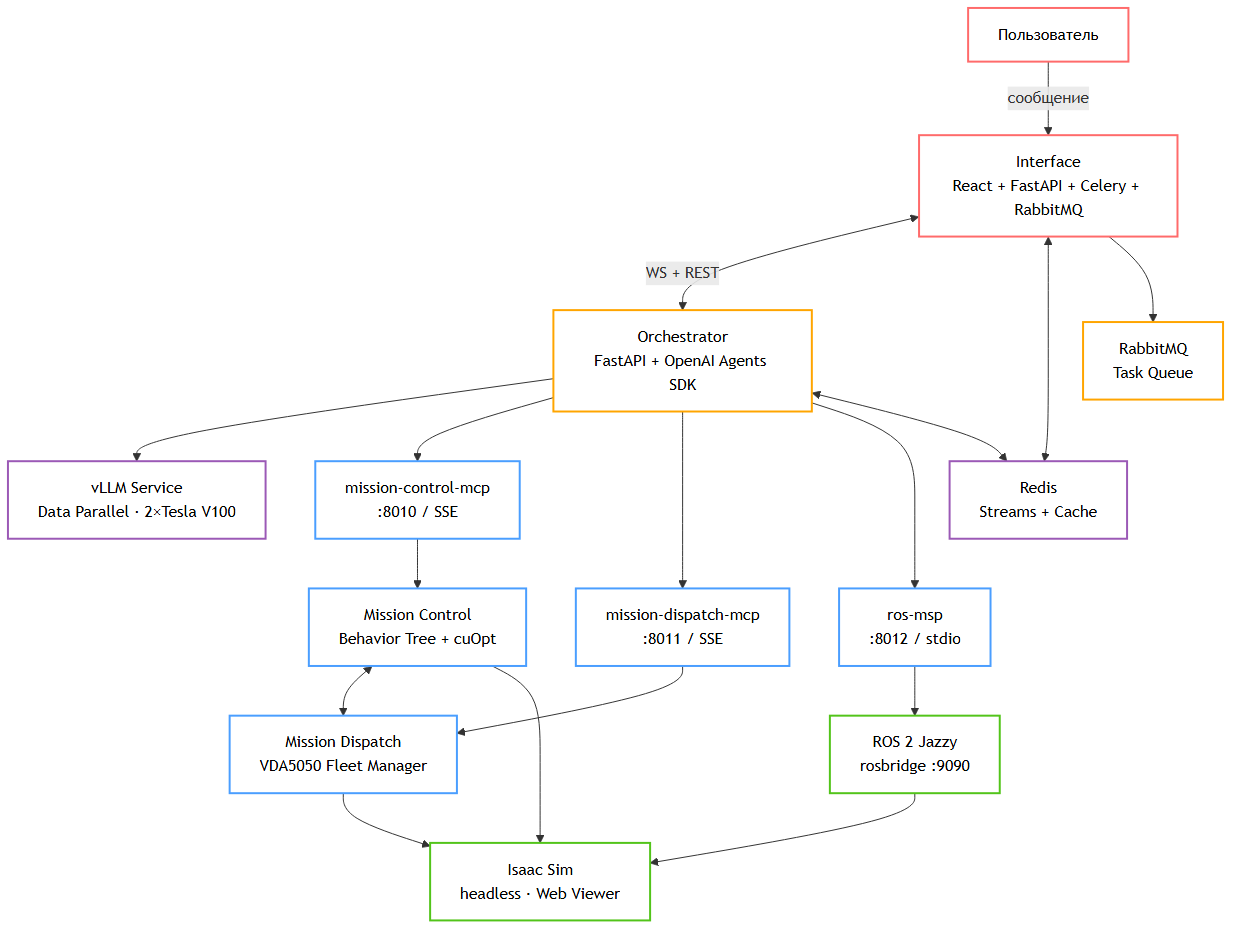
\includegraphics[width=0.95\textwidth]{img/fig_2_1_system_overview.png}
\caption{Общая схема взаимодействия компонентов системы AgentsSwarm}
\label{fig:system-overview}
\end{figure}

\section{Протокол взаимодействия агентов: Model Context Protocol}

\textbf{Model Context Protocol (MCP)}~\cite{mcp2024}~--- открытый стандарт для взаимодействия LLM-агентов с внешними инструментами и данными. Протокол определяет архитектуру клиент-сервер, где MCP-клиент (агент) вызывает tools, resources и prompts, предоставляемые MCP-сервером. Транспортный слой поддерживает два режима: SSE (Server-Sent Events) для HTTP-развёртывания и stdio для локальных процессов.

В системе AgentsSwarm реализованы три MCP-сервера с чёткими зонами ответственности:
\begin{itemize}
  \item \texttt{mission-control-mcp}~--- инструменты для работы с картой, waypoint-графом и статусами роботов (Mission Control API);
  \item \texttt{mission-dispatch-mcp}~--- инструменты для создания, управления и мониторинга миссий (Mission Dispatch API);
  \item \texttt{ros-msp}~--- инструменты для публикации в ROS~2 топики и чтения из них через rosbridge WebSocket~\cite{ros_mcp}.
\end{itemize}

MCP обеспечивает строгое разделение ответственности: агентный слой не зависит от конкретной реализации роботического контура и взаимодействует с ним исключительно через стандартизованный tool-интерфейс. Это позволяет заменять или расширять роботический контур без модификации кода оркестратора.

Зоны ответственности MCP-серверов показаны на рис.~\ref{fig:mcp-servers}.

\begin{figure}[H]
\centering
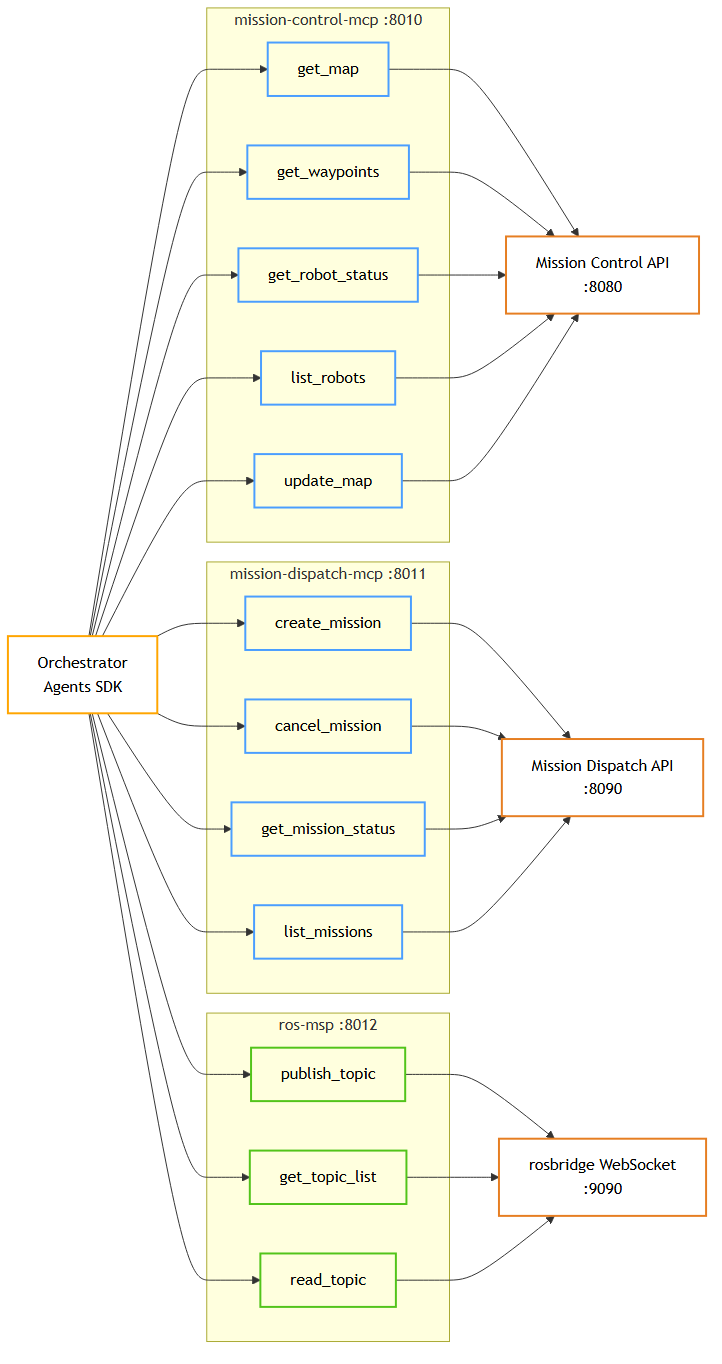
\includegraphics[height=0.75\textheight,keepaspectratio]{img/fig_2_2_mcp_servers.png}
\caption{Три MCP-сервера системы AgentsSwarm и их зоны ответственности}
\label{fig:mcp-servers}
\end{figure}

\section{Протокол управления флотом: VDA5050}

Стандарт VDA5050~\cite{vda5050} определяет JSON-структуры сообщений, передаваемых через MQTT-брокер:
\begin{itemize}
  \item \texttt{order}~--- задание для робота (последовательность узлов графа и рёбер с действиями);
  \item \texttt{state}~--- текущее состояние робота (позиция, статус, ошибки, уровень заряда);
  \item \texttt{connection}~--- статус подключения робота к fleet manager.
\end{itemize}

Маршрут команды в AgentsSwarm:
\begin{center}
  Orchestrator $\to$ MCP-сервер $\to$ Mission Dispatch API $\to$ MQTT $\to$ VDA5050 клиент $\to$ Isaac Sim
\end{center}

Mission Control принимает высокоуровневую задачу, строит Behavior Tree, запрашивает оптимальный маршрут у cuOpt и формирует VDA5050 order для Mission Dispatch. Mission Dispatch публикует order в MQTT-топик, VDA5050 клиент робота в Isaac Sim подписан на этот топик и исполняет команду.

Маршрут команды от пользовательского запроса до роботического контура показан на рис.~\ref{fig:command-route}.

\begin{landscape}
\begin{figure}[p]
\centering
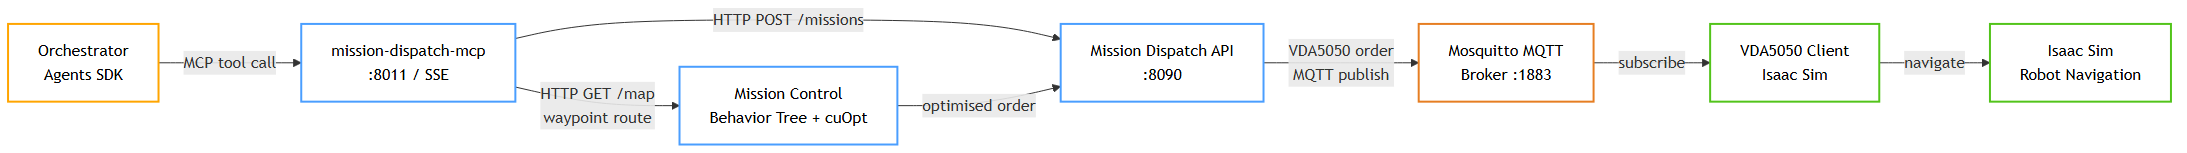
\includegraphics[width=0.5\linewidth, angle=270]{img/fig_2_3_command_route.png}
\caption{Маршрут команды: Orchestrator → MCP → Mission Dispatch → VDA5050 → робот}
\label{fig:command-route}
\end{figure}
\end{landscape}

\section{Агентная архитектура оркестратора}

Агентная архитектура оркестратора построена по иерархическому принципу: входящий запрос обрабатывается Router Agent, классифицирующим его по восьми категориям, после чего планировщик формирует последовательность исполняемых шагов.

\textbf{Router Agent} классифицирует запросы по категориям: \textit{general} (общие вопросы), \textit{robot\_info} (статусы роботов и диагностика), \textit{navigation} (задачи навигации), \textit{charging} (управление зарядкой), \textit{patrol} (патрульные маршруты), \textit{inspection} (инспекция объектов), \textit{fleet\_ops} (операции с флотом), \textit{swarm\_coord} (координация нескольких роботов). Классификация выполняется через LLM с детерминированными правилами приоритетов.

\textbf{Planner и PlanRunner} реализуют двухфазный алгоритм: на первой фазе строится план в виде последовательности именованных шагов с указанием \texttt{target\_robots} и зависимостей; на второй~--- шаги последовательно исполняются через агентов RobotInfo, MapAnalyst, Navigation, SwarmCoordinator и General либо через эвристический fallback в тестовом режиме.

\textbf{MapAnalyst} получает PNG-снимок карты от Mission Control, накладывает позиции роботов и передаёт изображение в vision-LLM для пространственного анализа сцены.

Категории Charging, Patrol, Inspection и FleetOps присутствуют в конфигурации маршрутизатора как расширяемые handoff-направления; в текущем исполняемом контуре PlanRunner основной набор шагов сводится к RobotInfo, MapAnalyst, Navigation, SwarmCoordinator и General.

Иерархия планирования и handoff-направлений приведена на рис.~\ref{fig:agent-hierarchy}.

\begin{figure}[H]
\centering
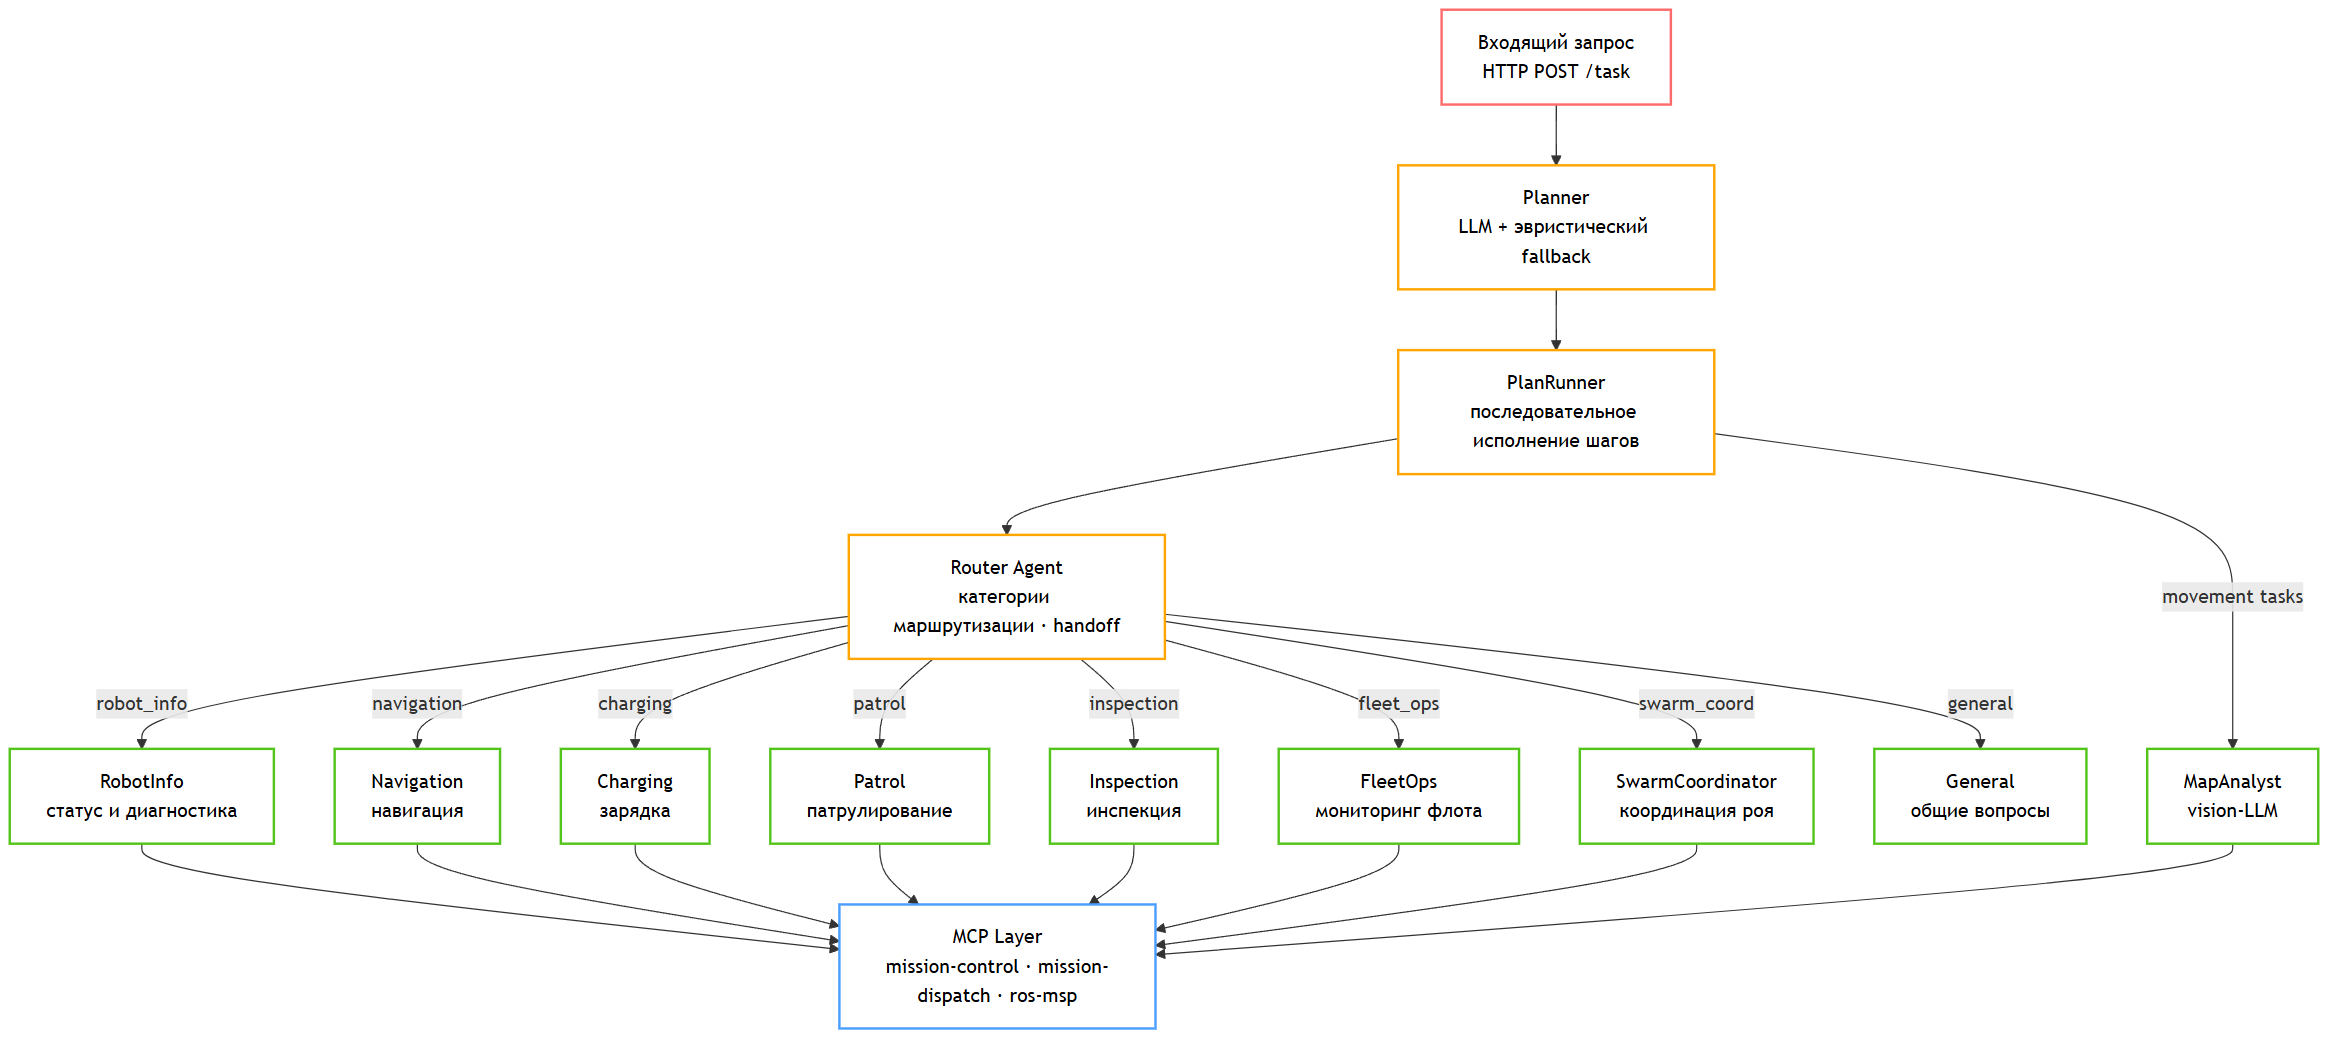
\includegraphics[width=0.95\textwidth]{img/fig_2_4_agents.png}
\caption{Планировщик, исполнитель шагов и специализированные агенты оркестратора}
\label{fig:agent-hierarchy}
\end{figure}

\section{Событийно-ориентированная потоковая модель}

Асинхронная потоковая модель Interface построена на Redis Stream как шине событий. Агент-воркер публикует события в поток \texttt{chat:\{thread\_id\}:stream} командой XADD; WebSocket-слой читает поток командой XREAD с блокирующим ожиданием и проталкивает события клиенту.

Жизненный цикл задачи: \textit{pending} $\to$ \textit{running} (первый чанк) $\to$ \textit{completed} или \textit{error}. Типы событий: \texttt{stream\_chunk}, \texttt{agent\_reply}, \texttt{routing\_event}, \texttt{tool\_event}, \texttt{error}.

Параллельный канал~--- REST-взаимодействие с оркестратором: SwarmOrchestratorAgent создаёт задачу через \texttt{POST /task}, затем инкрементально опрашивает \texttt{GET /task/\{id\}/events} и транслирует события в Redis Stream Interface, обеспечивая сквозную прозрачность агентного маршрута для пользователя.

Жизненный цикл задачи и потоковая модель событий показаны на рис.~\ref{fig:task-lifecycle}.

\begin{figure}[H]
\centering
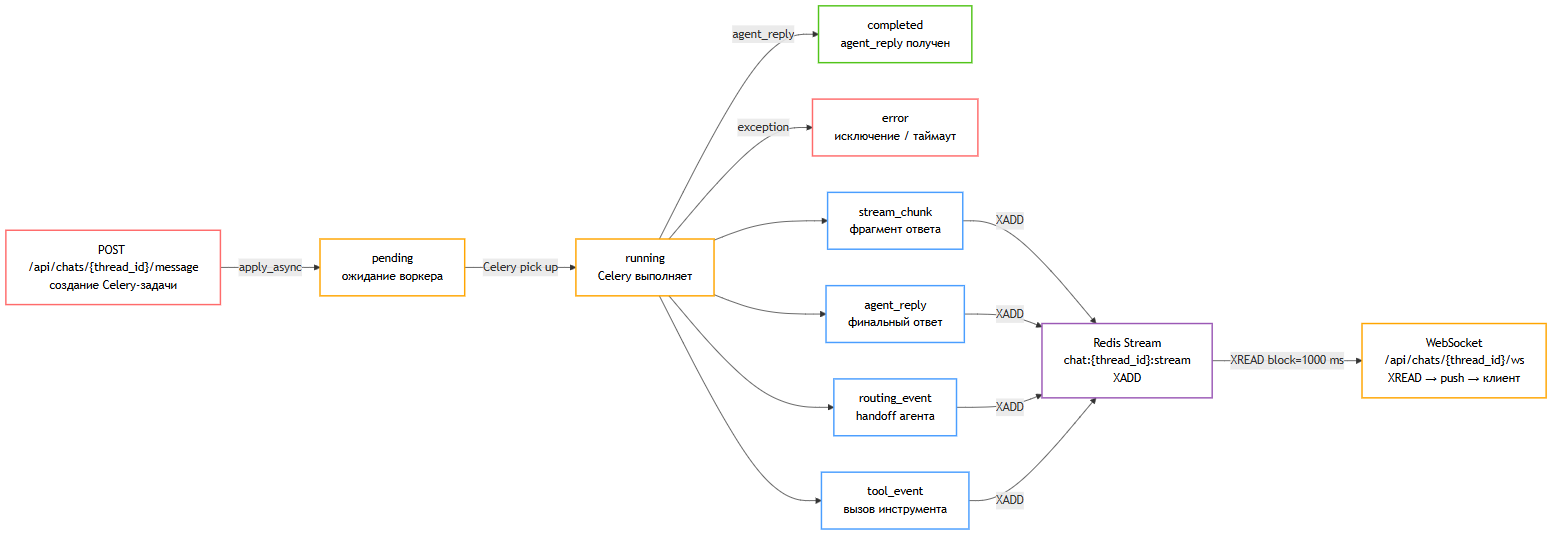
\includegraphics[width=0.95\textwidth]{img/fig_2_5_task_lifecycle.png}
\caption{Жизненный цикл задачи (pending → completed) и потоковая модель событий Redis Streams}
\label{fig:task-lifecycle}
\end{figure}

\section{Инфраструктура развёртывания}

Три машины разной конфигурации обслуживают различные подсистемы системы AgentsSwarm (Табл.~\ref{tab:infra}).

\begin{table}[H]
\caption{Технические характеристики вычислительной инфраструктуры}
\label{tab:infra}
\begin{tabular}{@{}>{\raggedright\arraybackslash}p{3.3cm}
                >{\raggedright\arraybackslash}p{2.4cm}
                >{\raggedright\arraybackslash}p{5.2cm}
                >{\raggedright\arraybackslash}p{3.7cm}@{}}
\toprule
\textbf{Машина} & \textbf{Провай\-дер} & \textbf{Конфигурация} & \textbf{Назначение} \\
\midrule
Симуляция & Selectel & 4 vCPU, 16~ГБ RAM, RTX~4090 (24~ГБ VRAM), Ubuntu 24.04 & Isaac Sim, ROS~2, Mission Control, Mission Dispatch \\
Микросервисы & Selectel & 4 vCPU, 8~ГБ RAM, 128~ГБ SSD, Ubuntu 24.04 & Interface, Orchestrator, Redis, RabbitMQ, MinIO, PostgreSQL \\
LLM-кластер & MTS Cloud & 2 узла × Tesla V100-PCIE 32~ГБ VRAM, Ubuntu 24.04 & vLLM Data Parallel (Qwen2.5-Instruct) \\
\bottomrule
\end{tabular}
\end{table}

Межсервисное взаимодействие: HTTP/REST (оркестратор $\leftrightarrow$ MCP, Interface $\leftrightarrow$ оркестратор), WebSocket (стриминг событий), MQTT (VDA5050), RPC gRPC (vLLM Data Parallel, порт 13345).

\section{Выводы и результаты по главе~2}

Спроектированная архитектура AgentsSwarm обеспечивает чёткое разделение ответственности между компонентами: пользовательский слой (Interface) изолирован от роботического контура (Mission Control/Dispatch/Isaac Sim) через двухступенчатый агентный барьер (Interface-агенты $\to$ Orchestrator-агенты $\to$ MCP-серверы).

Принципиальной новизной по сравнению с рассмотренными аналогами является интеграция LLM-слоя с промышленным VDA5050-контуром через стандартизованный MCP-протокол. OpenRMF~\cite{openrmf} и аналогичные fleet management системы требуют формального задания задачи через API; AgentsSwarm принимает произвольный запрос на естественном языке и транслирует его в исполнимую последовательность VDA5050-команд. Событийно-ориентированная потоковая модель на Redis Streams обеспечивает наблюдаемость сквозного контура выполнения задачи для пользователя в реальном времени.

% ============================================================
%  ГЛАВА 3. РЕАЛИЗАЦИЯ КОМПОНЕНТОВ
% ============================================================
\chapter{Реализация компонентов системы}

\section{Симуляционная среда: NVIDIA Isaac Sim и ROS~2 Workspace}

Симуляционная среда построена на базе NVIDIA Isaac Sim 4.5 в headless-режиме с Web Viewer для удалённого наблюдения~\cite{nvidia2024isaac,isaacsim_multirobot}. Сцена Carter Warehouse содержит несколько роботов Carter с уникальными ROS~2-пространствами имён (namespaces), что позволяет независимо управлять каждым роботом через единый ROS~2 DDS-мост.

Запуск осуществляется через Docker Compose стек: контейнер Isaac Sim монтирует GPU, обеспечивает доступ к драйверам CUDA и публикует Web Viewer на порту 8211. Конфигурация Action Graph задаёт параметры синтетической камеры, публикует RGB- и depth-изображения в ROS~2-топики и запускает \texttt{isaac\_ros\_mission\_client}~--- официальный пакет NVIDIA, реализующий VDA5050 клиент для флота роботов~\cite{isaacros_packages}.

ROS~2 Jazzy workspace собирается из форка \texttt{isaac\_ros\_common}, дополненного пакетами для отображения occupancy map, публикации costmap и rosbridge-сервером~\cite{isaacros2024,isaacsim_ros_ws,ros2jazzy}. Rosbridge WebSocket (порт 9090) обеспечивает доступ к ROS~2-топикам для MCP-сервера без необходимости установки полного стека ROS~2 на машине оркестратора~\cite{rosbridge}.

\textbf{Occupancy map} генерируется из ортогонального вида сцены Isaac Sim, сохраняется в формате PNG и обновляется в Mission Control через маршрут API \texttt{/map/update\_robot}. На основе карты Mission Control строит waypoint graph~--- ориентированный граф навигационных узлов, по которому cuOpt рассчитывает оптимальные маршруты.

Интеграция Isaac Sim, ROS~2 и VDA5050 показана на рис.~\ref{fig:isaac-ros}; пример waypoint graph сцены Carter Warehouse приведён на рис.~\ref{fig:map-waypoints}.

\begin{figure}[H]
\centering
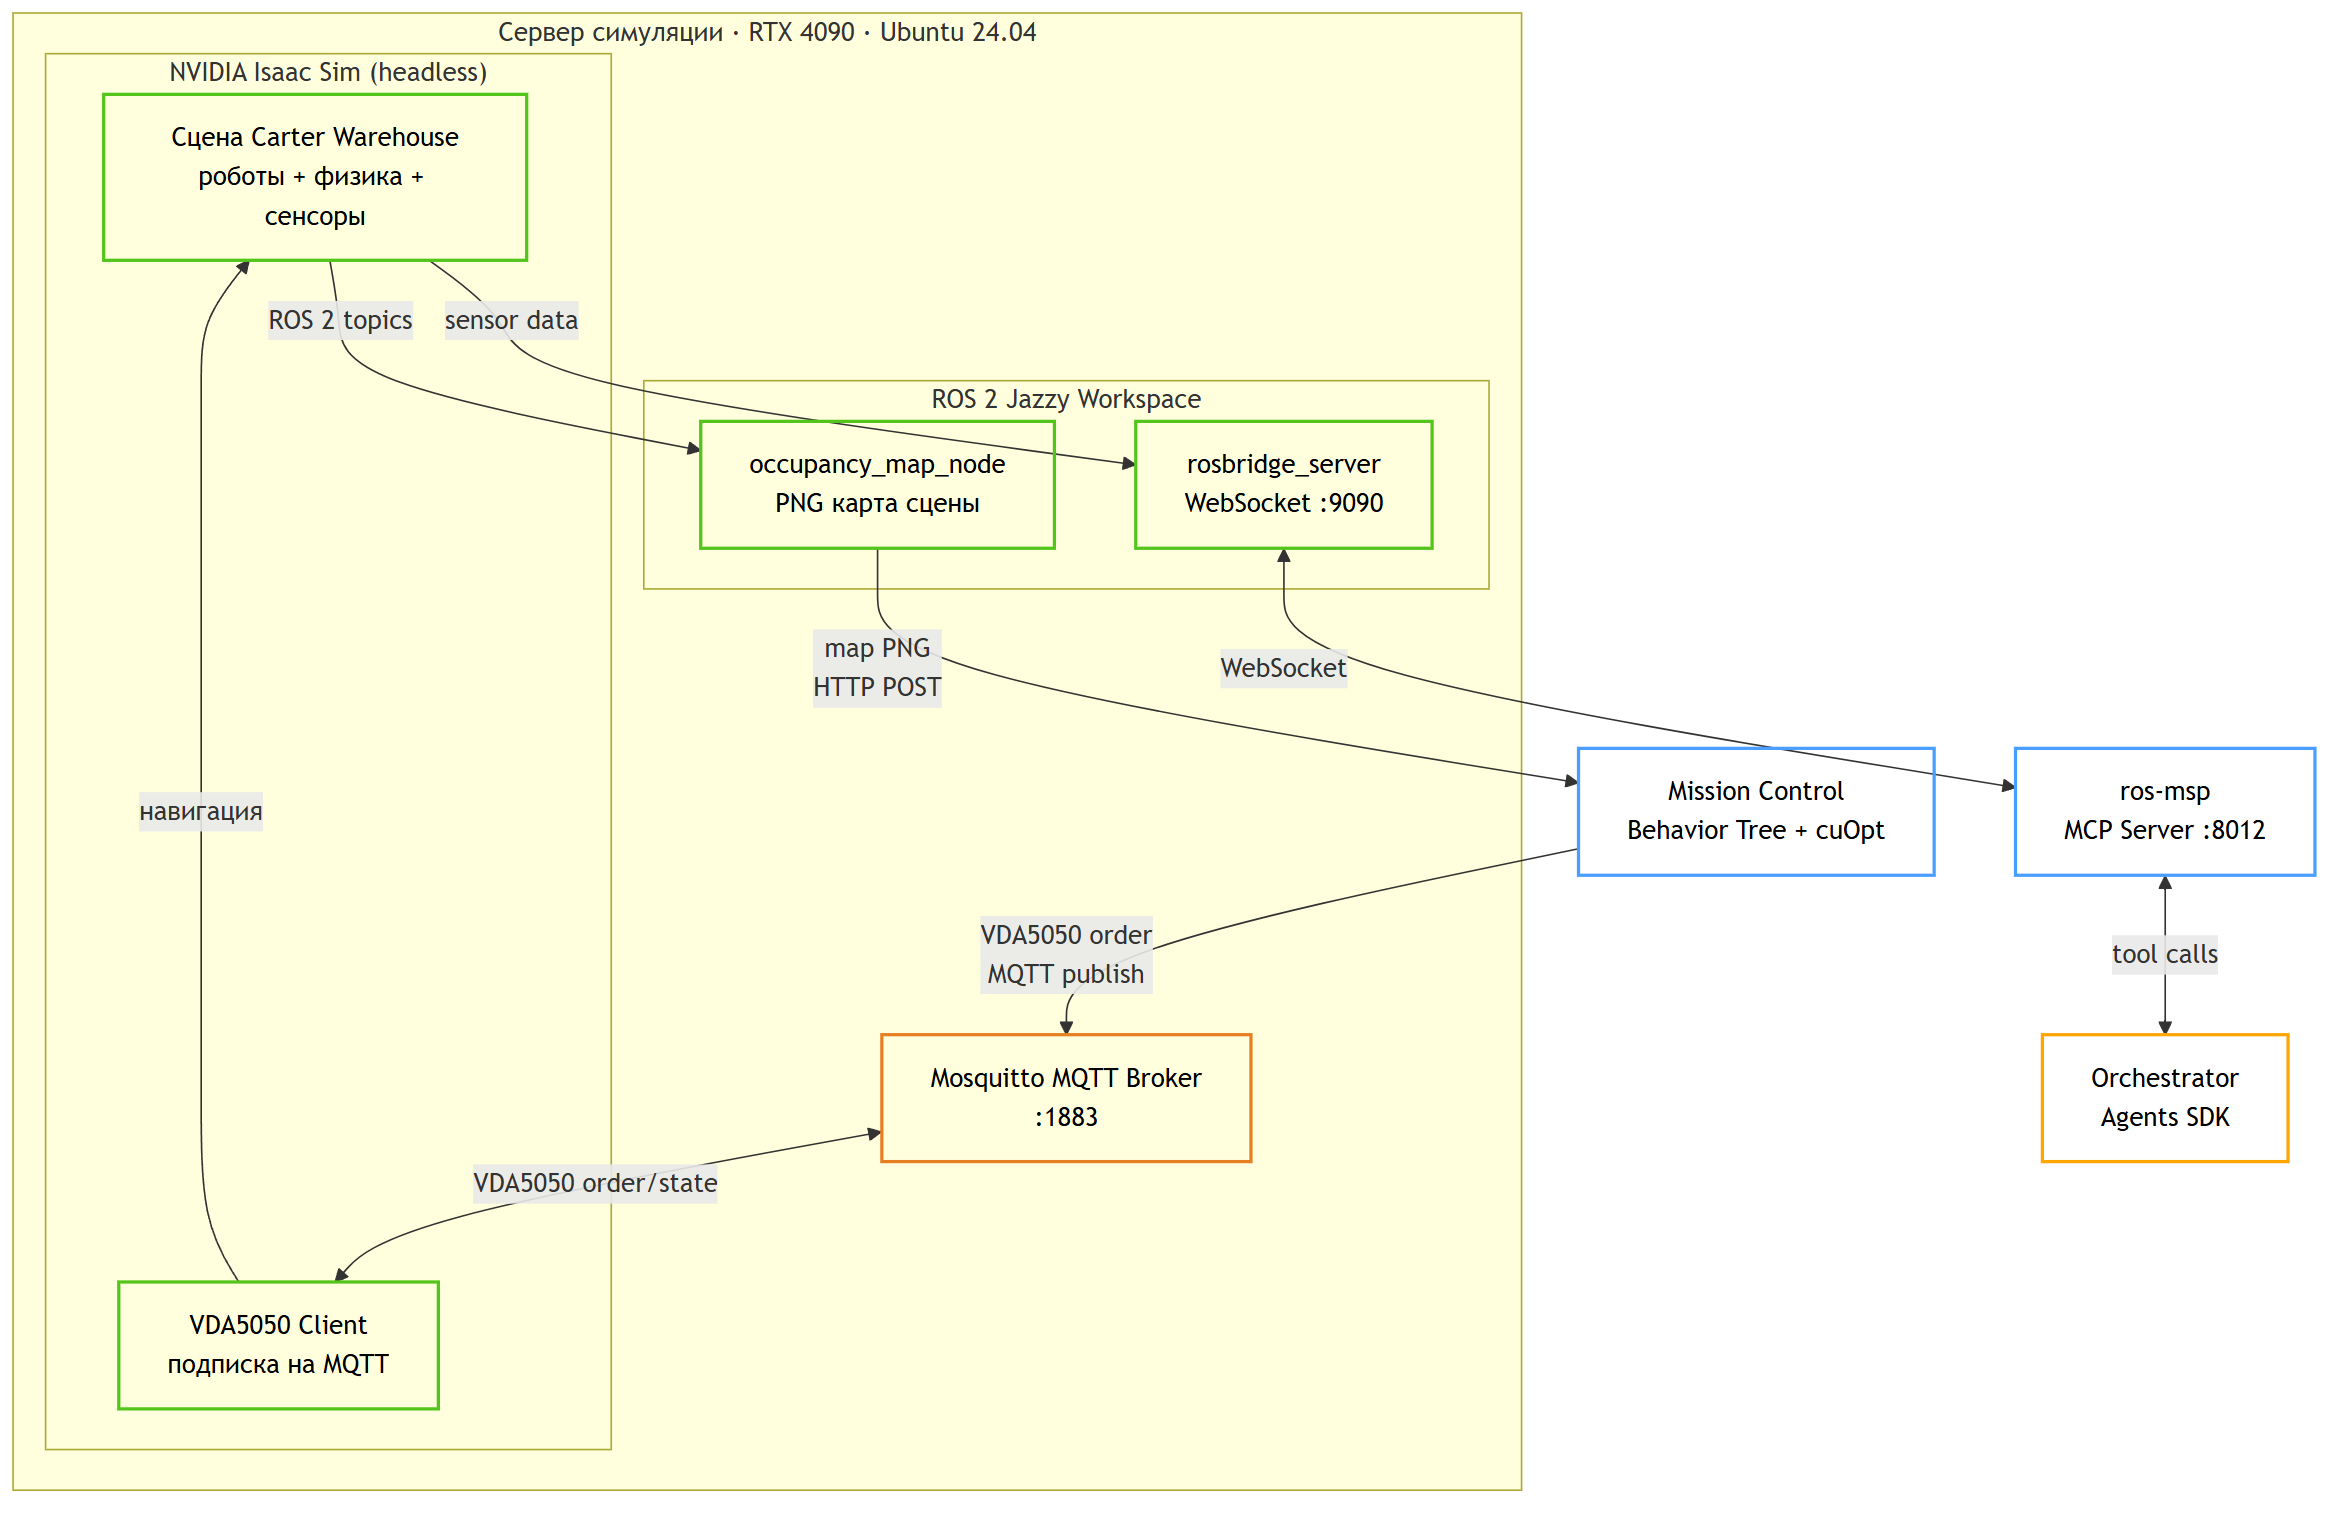
\includegraphics[width=0.95\textwidth]{img/fig_3_1_isaac_ros.png}
\caption{Схема интеграции Isaac Sim, ROS~2 и VDA5050 в симуляционном контуре}
\label{fig:isaac-ros}
\end{figure}

\begin{figure}[H]
\centering
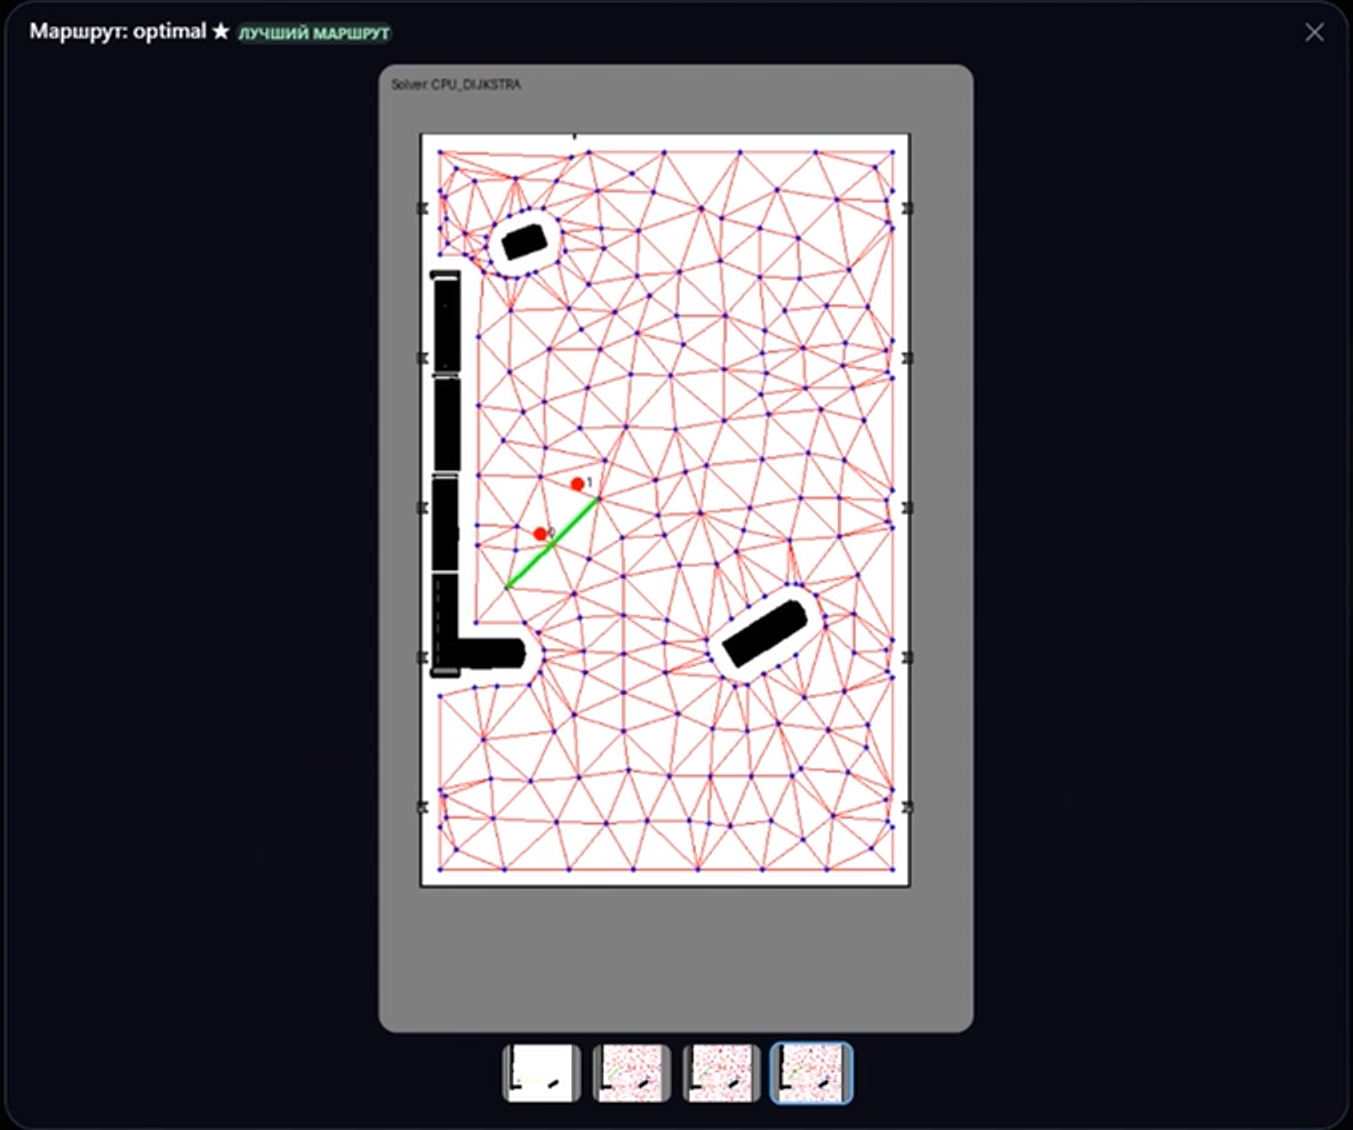
\includegraphics[width=0.95\textwidth]{img/fig_3_2_map_waypoints.png}
\caption{Occupancy map и waypoint graph сцены Carter Warehouse}
\label{fig:map-waypoints}
\end{figure}

\section{Mission Control: форк NVIDIA и авторские доработки}

Официальный репозиторий NVIDIA Mission Control реализует централизованный fleet manager для VDA5050-совместимых роботов с Behavior Tree планировщиком и поддержкой cuOpt для оптимизации маршрутов~\cite{missioncontrol,cuopt}. При развёртывании оригинального кода были выявлены критические ошибки.

\textbf{Проблема~1: несоответствие маршрута обновления карты.} Оригинальный код вызывал \texttt{/push\_map}, тогда как Mission Control API использует \texttt{/map/update\_robot} и \texttt{/map/metadata}. Исправление потребовало анализа HTTP-трафика между компонентами и корректировки маршрутизации внутри Mission Control.

\textbf{Проблема~2: устаревший синтаксис Pydantic v1.} Модуль \texttt{waypoint\_selection\_ui} использовал декораторы-валидаторы, несовместимые с Pydantic v2. Исправление состояло в замене на актуальный синтаксис \texttt{@field\_validator}.

Стабилизация Docker-стека включала корректировку порядка запуска зависимых сервисов (cuOpt, Mosquitto, PostgreSQL) и проверку health-check проб для корректной инициализации. После всех исправлений Mission Control успешно принимает задания от оркестратора, строит Behavior Tree и публикует VDA5050 order в Mosquitto.

\section{Mission Dispatch: форк NVIDIA и авторские доработки}

Mission Dispatch реализует очередь миссий и двустороннее VDA5050-взаимодействие между fleet manager и роботами~\cite{missiondispatch}. В оригинальном коде обнаружена проблема с устаревшим маршрутом в пакете \texttt{packages/controllers/server}: запросы возвращали 404, нарушая сквозное взаимодействие.

Дополнительно выявлена некорректная конфигурация MQTT-хоста: Mission Dispatch использовал жёстко заданный \texttt{localhost} вместо имени сервиса Docker Compose (\texttt{mosquitto}), что препятствовало работе в контейнеризованном окружении. После исправления двух ошибок проведена сквозная верификация цепочки:

\begin{center}
Isaac Sim $\to$ VDA5050 клиент $\to$ Mosquitto $\to$ Mission Dispatch $\to$ Mission Control $\to$ Behavior Tree $\to$ VDA5050 order $\to$ Isaac Sim
\end{center}

\section{MCP-серверы: переработка официальных реализаций}

Три MCP-сервера обеспечивают агентам оркестратора доступ к роботическому контуру через стандартизованный интерфейс инструментов~\cite{mcp2024,fastmcp}. Исходные реализации MCP-серверов NVIDIA представляли прототипы с нереализованными служебными маршрутами и синхронной моделью вызовов.

\textbf{Переход на асинхронную модель.} Все инструменты переписаны на \texttt{async def} с \texttt{httpx.AsyncClient} для HTTP и \texttt{websockets} для rosbridge-соединений. Это обеспечивает корректную работу с event loop без блокировки при параллельных вызовах агентов.

\textbf{mission-control-mcp} предоставляет инструменты верхнего уровня Mission Control. Для миссий зарегистрированы обработчики навигации, зарядки и undock; основной навигационный вызов в коде имеет имя \texttt{submit\_navigation\_mission}. Для карт используются \texttt{get\_map\_info}, \texttt{list\_available\_maps}, \texttt{select\_map}, \texttt{deploy\_map\_to\_robot} и \texttt{visualize\_route}. Отдельно реализованы проверка соединения, операции с detected objects, apriltags, objectives и pick-and-place. Нереализованные обработчики заменены рабочими служебными маршрутами, необходимыми для корректной инициализации Mission Control.

\textbf{mission-dispatch-mcp} предоставляет инструменты статуса и управления исполнением. Группа мониторинга покрывает статусы роботов и миссий, свободных роботов, сводку флота, проверку исправности, очередь миссий и последние отказы; ключевые имена в коде~--- \texttt{get\_robot\_status}, \texttt{get\_mission\_status}, \texttt{get\_idle\_robots}, \texttt{check\_robot\_health}. Группа управления включает \texttt{dispatch\_mission}, \texttt{dispatch\_route}, \texttt{cancel\_mission} и \texttt{cancel\_active\_missions}. Исправлены несовместимые адреса API.

\textbf{ros-msp} предоставляет группы FastMCP-инструментов для ROS~2 через rosbridge~\cite{ros_mcp,rosbridge}: подключение к роботу и ping, топики, сервисы, actions, параметры, узлы, сохранённые изображения и верифицированные спецификации роботов. В коде это соответствует инструментам \texttt{connect\_to\_robot}, \texttt{ping\_robots}, \texttt{get\_topics}, \texttt{subscribe\_once}, \texttt{publish\_once}, \texttt{get\_services}, \texttt{call\_service}, \texttt{get\_actions}, \texttt{send\_action\_goal} и смежным инструментам чтения метаданных. Сервер устанавливает постоянное WebSocket-соединение с rosbridge при инициализации.

\textbf{Динамический выбор транспорта} реализован через переменную окружения \texttt{MCP\_TRANSPORT}: при значении \texttt{sse} сервер запускается как HTTP-приложение; при \texttt{stdio}~--- как локальный процесс со стандартными потоками. Один и тот же код используется для локального тестирования и промышленного развёртывания.

Схема выбора транспорта MCP приведена на рис.~\ref{fig:mcp-transport}.

\begin{figure}[H]
\centering
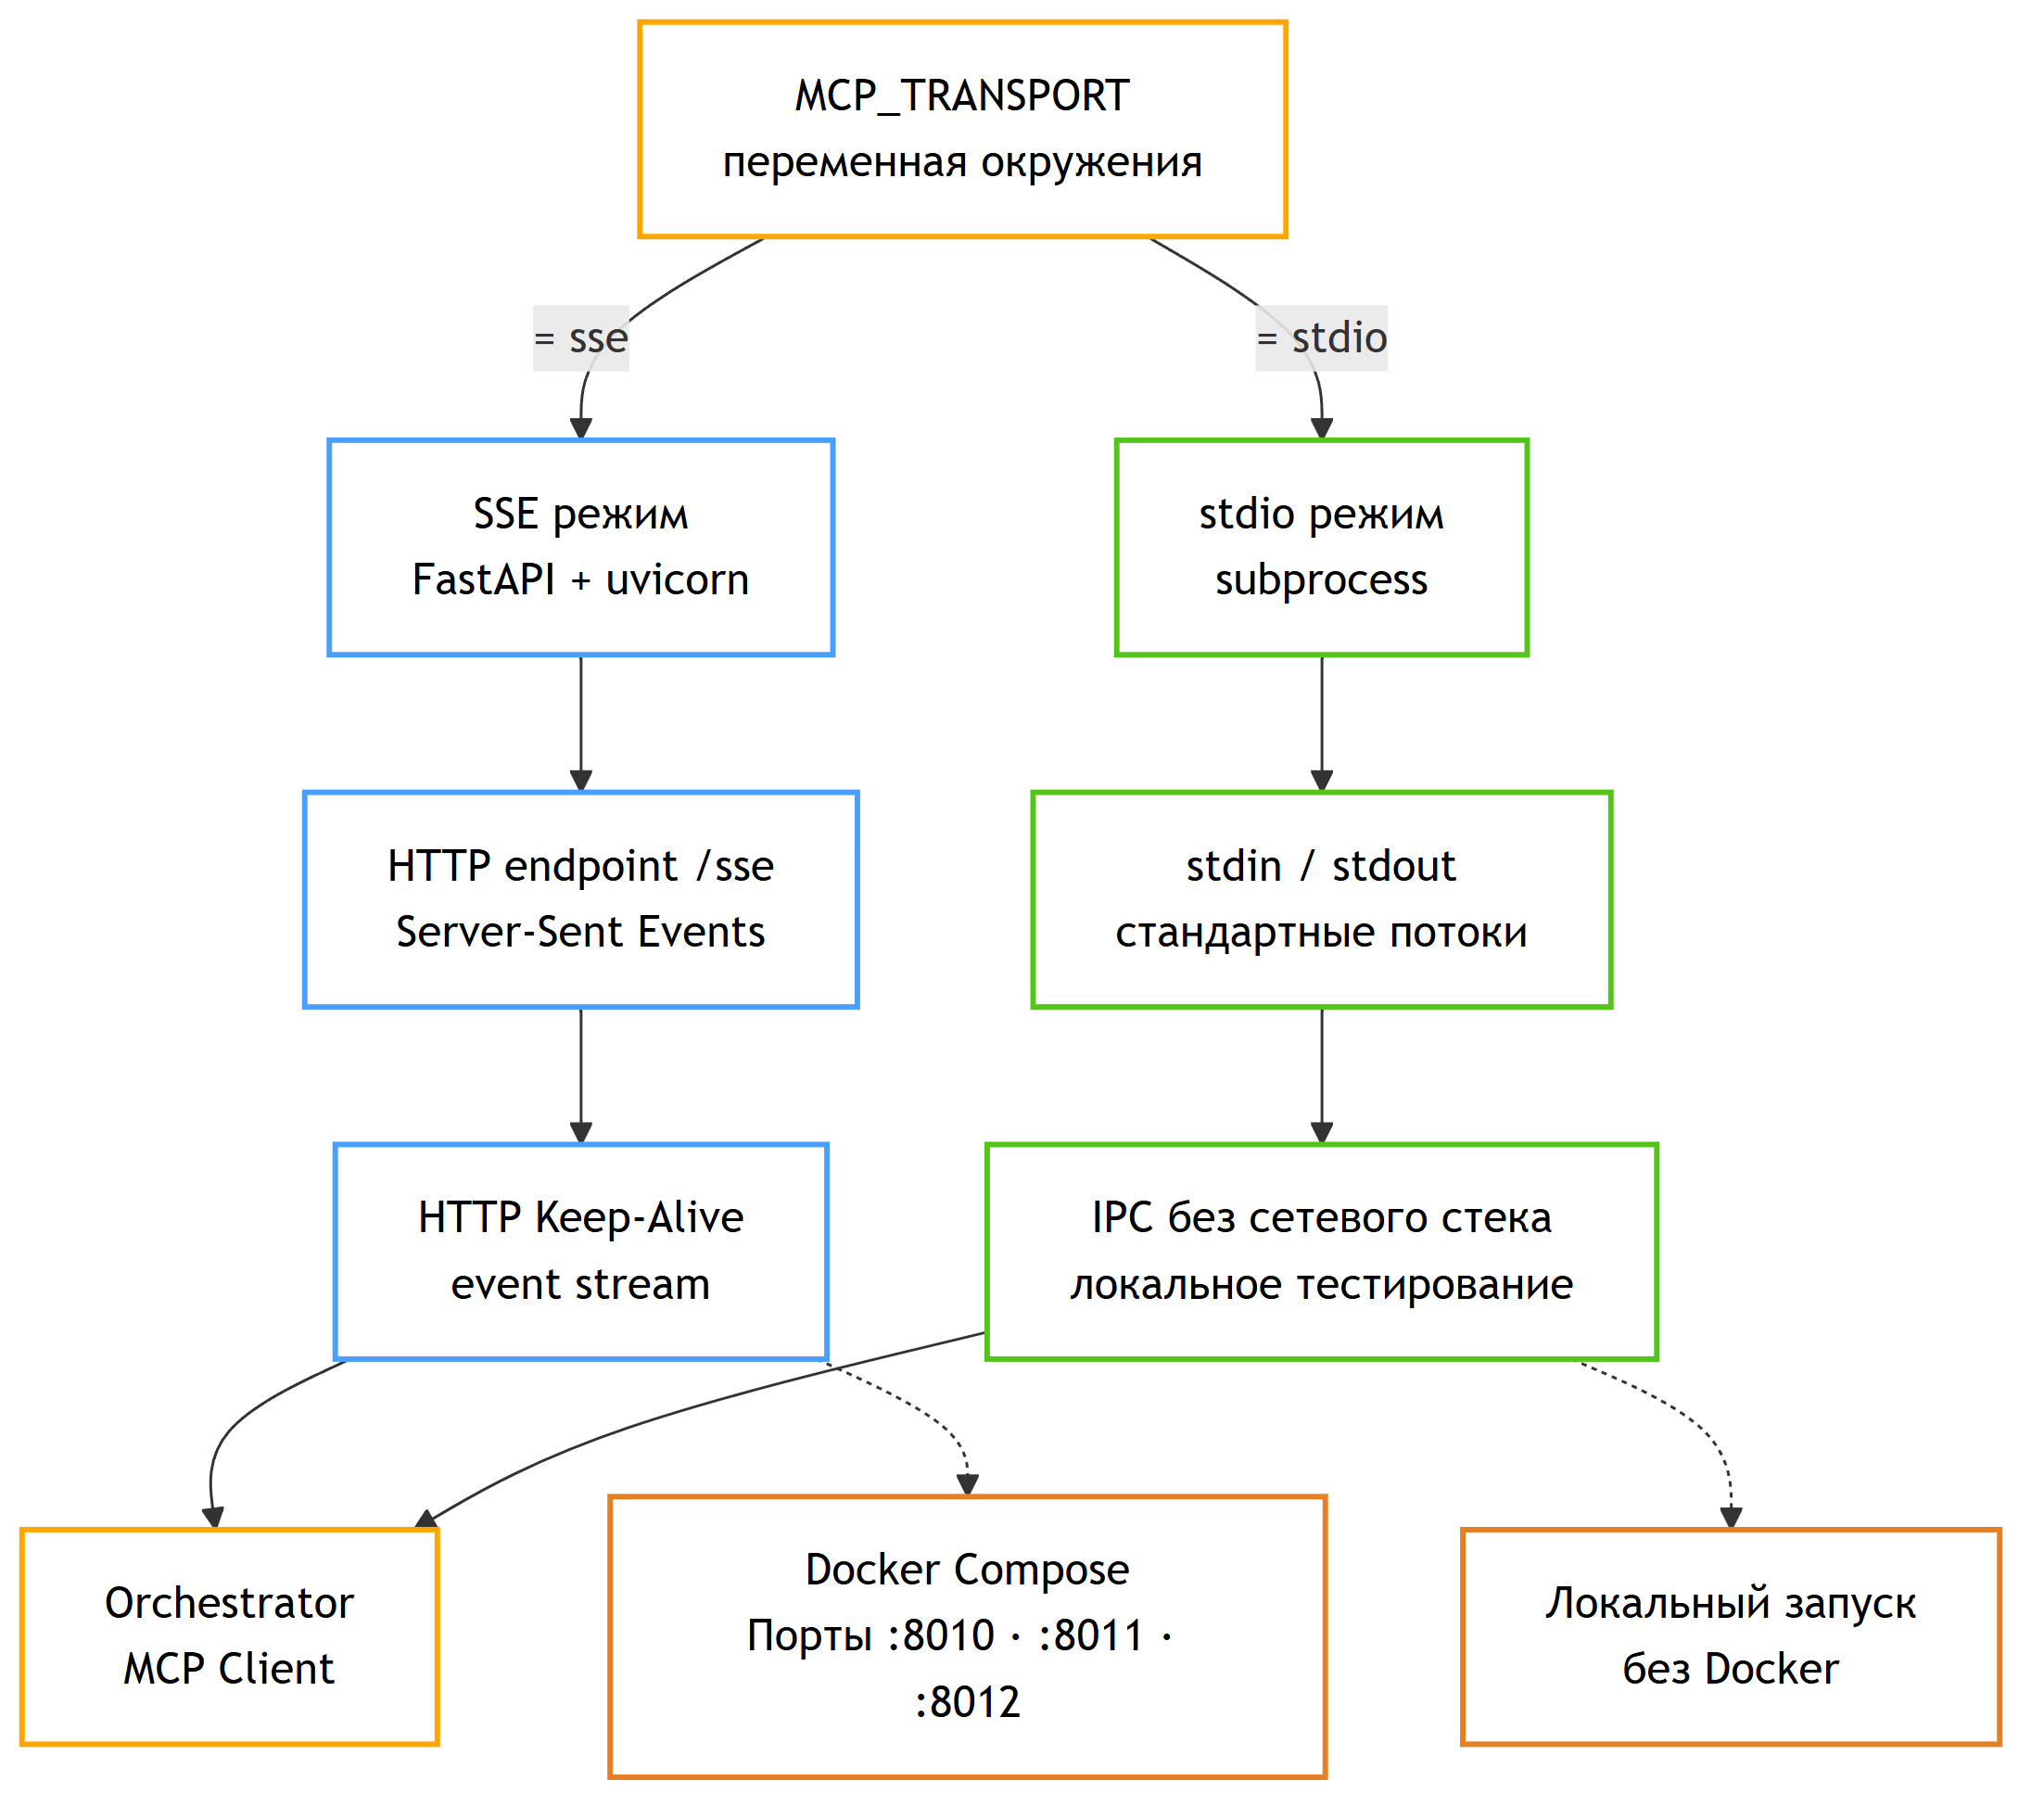
\includegraphics[width=0.90\textwidth]{img/fig_3_3_mcp_transport.png}
\caption{Динамический выбор транспорта MCP: SSE (HTTP) и stdio режимы через переменную окружения}
\label{fig:mcp-transport}
\end{figure}

\section{vLLM Service: авторский сервис инференса}

Авторский vLLM-сервис обеспечивает инференс Qwen2.5-Instruct в режиме Data Parallel на двух физически разных узлах~\cite{vllm_project,qwen25_model}.

\textbf{Архитектура Data Parallel:} узел~0 (координатор, rank~0) принимает HTTP-запросы, а узел~1 (воркер, rank~1) подключается к нему через RPC-канал на порту 13345. Конфигурация задаётся параметрами \texttt{data\_parallel\_size}, \texttt{data\_parallel\_rank}, \texttt{data\_parallel\_address} и \texttt{data\_parallel\_rpc\_port}; внутри каждого узла используется \texttt{tensor\_parallel\_size=1}. Суммарно доступно 64~ГБ VRAM, что позволяет развернуть крупную Qwen2.5-Instruct модель с заполнением $\approx$~90\% памяти.

Конфигурация узлов задаётся через окружение: адрес и порт HTTP-сервиса, доля доступной GPU-памяти, размер и ранг Data Parallel, адрес координатора, RPC-порт Data Parallel и локальный размер Tensor Parallel. В скриптах развёртывания эти значения передаются в vLLM через переменные семейства \texttt{VLLM\_*}; для рассматриваемого стенда используются Data Parallel size~2, RPC-порт 13345, заполнение GPU-памяти 0.90 и Tensor Parallel size~1.

Скрипты \texttt{deploy.sh} (Linux) и \texttt{deploy.bat} (Windows) автоматизируют: запуск Docker-контейнера vLLM с монтированием GPU и кэша модели; ожидание готовности \texttt{/health}; smoke-тест с тестовым промптом. Сервис полностью совместим с OpenAI Python SDK~--- требуется лишь установить \texttt{base\_url} и \texttt{api\_key="EMPTY"}.

Развёртывание vLLM Data Parallel показано на рис.~\ref{fig:vllm-dp}.

\begin{figure}[H]
\centering
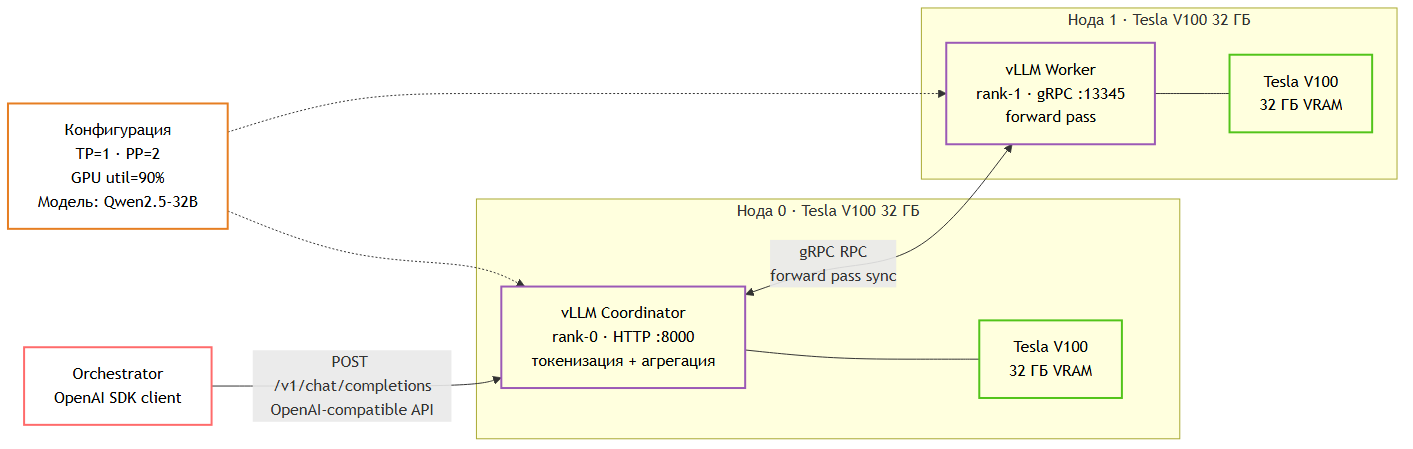
\includegraphics[width=0.90\textwidth]{img/fig_3_4_vllm_dp.png}
\caption{Архитектура vLLM Data Parallel: координатор (rank-0) и воркер (rank-1), связанные через gRPC}
\label{fig:vllm-dp}
\end{figure}

\section{Orchestrator: главный интеллектуальный микросервис}

Оркестратор~--- основной интеллектуальный сервис системы AgentsSwarm, реализованный на FastAPI с lifespan-менеджером (срез v0.5.6, 61~коммит).

\textbf{Структура приложения.} FastAPI-приложение предоставляет системный маршрут \texttt{/health}, маршрут постановки задачи \texttt{/task} и семейство маршрутов жизненного цикла \texttt{/task/\{task\_id\}/...}: \texttt{status}, \texttt{plan}, \texttt{logs}, \texttt{cancel}, \texttt{events}, \texttt{run}, \texttt{replan}. Поток событий отдаётся через WebSocket \texttt{/ws/task/\{task\_id\}}. Зависимости (SessionManager, StreamCollector, MCP-клиенты) регистрируются через Depends и инициализируются при старте lifespan.

\textbf{Агентная архитектура.} Агенты оркестратора создаются через OpenAI Agents SDK~\cite{openai_agents} и конфигурируются системными промптами:
\begin{itemize}
  \item \textit{Router}~--- классификация запросов по 8 категориям;
  \item \textit{RobotInfo}~--- статусы роботов, батарея, позиция и ROS~2-диагностика;
  \item \textit{MapAnalyst}~--- vision-LLM для пространственного анализа карты;
  \item \textit{Navigation}~--- навигационные команды, отмена активных миссий и контроль исполнения;
  \item \textit{SwarmCoordinator}~--- координация нескольких роботов;
  \item \textit{General}~--- ответы на общие вопросы без вызова роботических инструментов.
\end{itemize}

\textbf{Интеграция OpenAI Agents SDK.} Исполнитель использует \texttt{Runner.run\_streamed(agent, input=..., run\_config=..., max\_turns=...)} и читает асинхронный поток событий SDK. StreamCollector присваивает каждому событию порядковый номер (seq), буферизует его в памяти по \texttt{task\_id} и отдаёт накопленные события через \texttt{GET /task/\{task\_id\}/events} либо WebSocket \texttt{/ws/task/\{task\_id\}}.

\textbf{SessionManager} хранит историю диалога и кэш MCP-результатов в контексте задачи: при наличии \texttt{REDIS\_URL} данные сохраняются в Redis hash, при недоступности Redis используется in-memory fallback. Явный TTL для сессий в текущей реализации не задан.

\textbf{Guardrails} реализованы как слой валидации: входящий запрос проверяется на пустоту и чрезмерную длину, а результат маршрутизатора нормализуется к разрешённым категориям \textit{robot\_info}, \textit{navigation}, \textit{swarm\_coord} и \textit{general}. Невалидный результат переводится в fallback-ветку без прерывания сессии.

Retry с экспоненциальным backoff и jitter применяется для сетевых операций: общая утилита retry использует по умолчанию 3 попытки с базовой задержкой 0{,}1~с, а PlanRunner повторяет неуспешный handoff до двух попыток с задержкой 0{,}05~с.

Структура FastAPI-приложения оркестратора показана на рис.~\ref{fig:orchestrator-app}; отдельная схема StreamCollector приведена на рис.~\ref{fig:streamcollector}.

\begin{figure}[H]
\centering
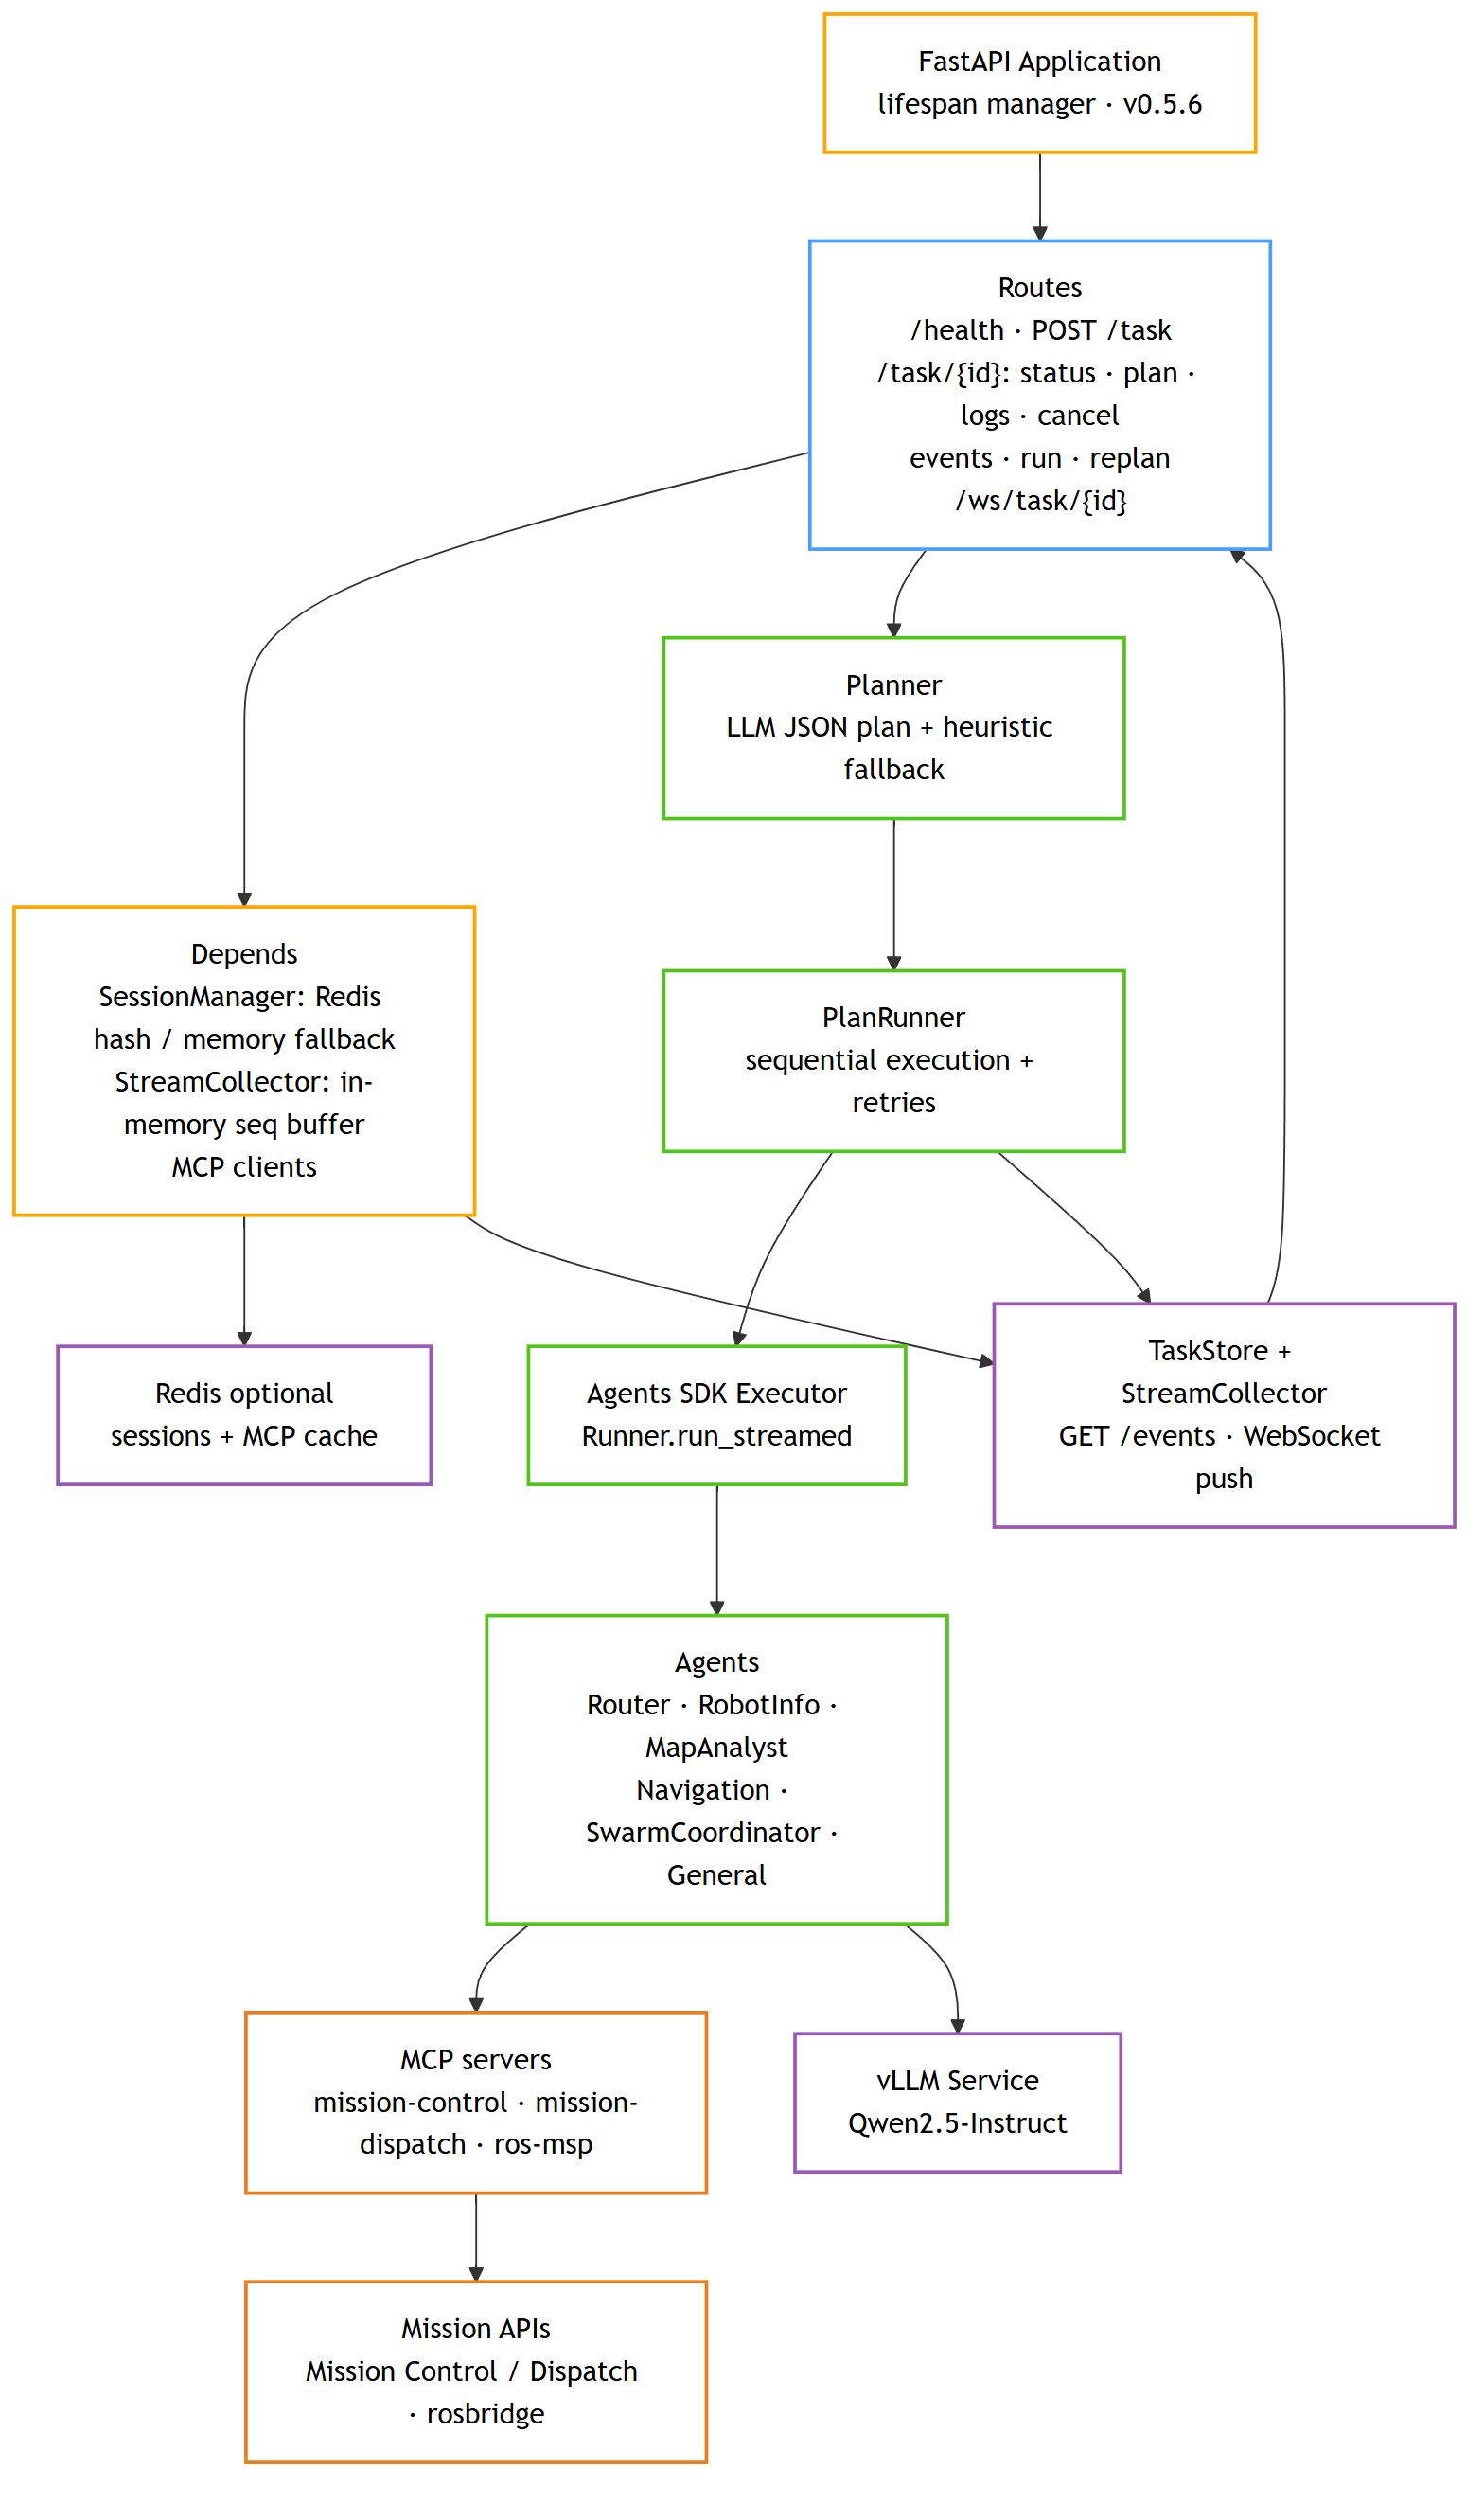
\includegraphics[height=0.72\textheight,keepaspectratio]{img/fig_3_5_orchestrator_app.png}
\caption{Структура FastAPI-приложения оркестратора: роутеры, зависимости и агентный слой}
\label{fig:orchestrator-app}
\end{figure}

\begin{figure}[H]
\centering
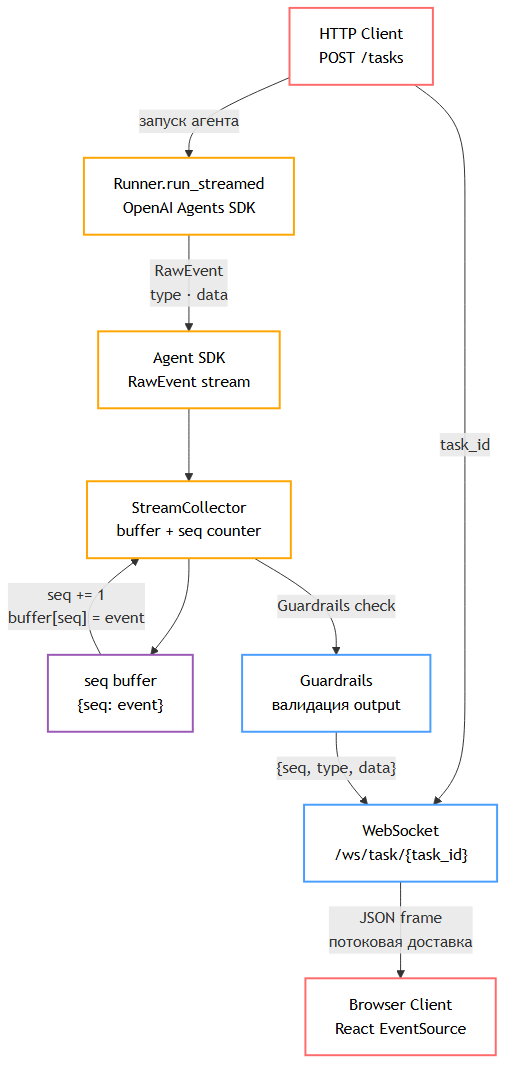
\includegraphics[height=0.72\textheight,keepaspectratio]{img/fig_3_6_streamcollector.png}
\caption{StreamCollector: seq-нумерация событий Agents SDK и выдача через polling/WebSocket}
\label{fig:streamcollector}
\end{figure}

\section{Interface: веб-платформа управления}

Interface~--- веб-портал для взаимодействия пользователя с системой AgentsSwarm (v0.5.0, 168~коммитов). Компонент разработан как самостоятельный сервис. Исходный код проекта AgentsSwarm опубликован в репозитории~\cite{agentsswarm_repo}.

\subsection{Общая архитектура и стек}

Бэкенд реализован по clean architecture: слои \textit{domain} (сущности и интерфейсы), \textit{application} (ChatService, ChatJobOrchestrator, AgentExecutionService), \textit{infrastructure} (PostgreSQL/SQLAlchemy, Redis, MinIO), \textit{api} (FastAPI роутеры, WebSocket-слой). Docker Compose предоставляет dev-стек (hot-reload) и prod-стек (Nginx + Gunicorn).

Архитектура Interface показана на рис.~\ref{fig:interface-arch}.

\begin{figure}[H]
\centering
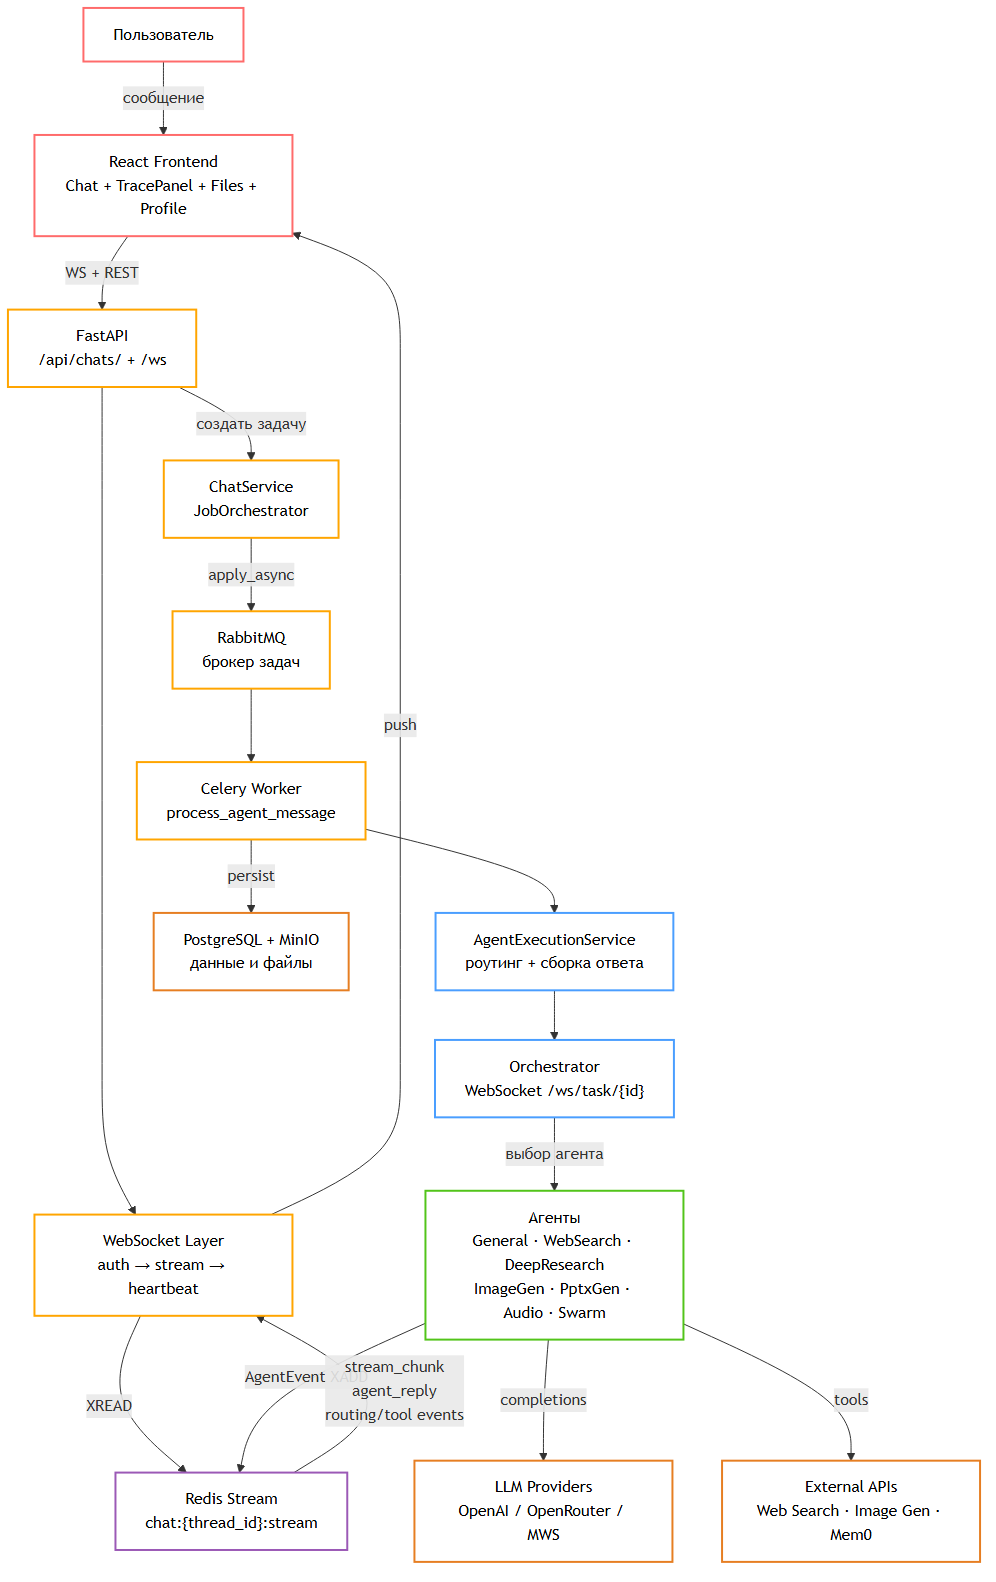
\includegraphics[width=0.95\textwidth]{img/fig_3_7_interface_arch.png}
\caption{Архитектура компонента Interface: React-фронтенд, FastAPI-бэкенд, Celery-воркеры и Redis Streams}
\label{fig:interface-arch}
\end{figure}

\subsection{Backend: агенты и обработка задач}

ChatJobOrchestrator и агентный pipeline маршрутизируют задачу к одному из семи агентов (Табл.~\ref{tab:iface-agents}):

\begin{table}[H]
\caption{Специализированные агенты компонента Interface и ключи их регистрации}
\label{tab:iface-agents}
\begin{tabular}{p{4.7cm}p{8.3cm}}
\toprule
\textbf{Ключ агента} & \textbf{Описание} \\
\midrule
\texttt{general} & Универсальный LLM-чат (Qwen2.5-Instruct) \\
\texttt{web\_search} & Поиск в интернете с агрегацией результатов \\
\texttt{deep\_research} & Многоитерационное глубокое исследование темы \\
\texttt{image\_gen} & Генерация изображений через внешний Image API \\
\texttt{pptx\_gen} & Создание PPTX-презентаций по шаблону \\
\texttt{audio\_transcribe} & Транскрипция аудио через Whisper \\
\texttt{swarm\_orchestrator} & Создание задачи в Orchestrator через REST и инкрементальный polling \texttt{/task/\{id\}/events} \\
\bottomrule
\end{tabular}
\end{table}

Celery-задача \texttt{process\_agent\_message} запускается при получении сообщения. В ходе выполнения агент публикует события в Redis Stream \texttt{chat:\{thread\_id\}:stream} через XADD.

\subsection{Потоковая модель: Redis Streams и WebSocket}

WebSocket-обработчик в FastAPI читает Redis Stream через XREAD с блокирующим ожиданием \texttt{block=1000} и проталкивает каждое событие клиенту. Heartbeat-механизм по умолчанию каждые 5~с отправляет JSON-сообщение для поддержания соединения.

Путь событий через Redis Stream и WebSocket приведён на рис.~\ref{fig:redis-stream}.

\begin{figure}[H]
\centering
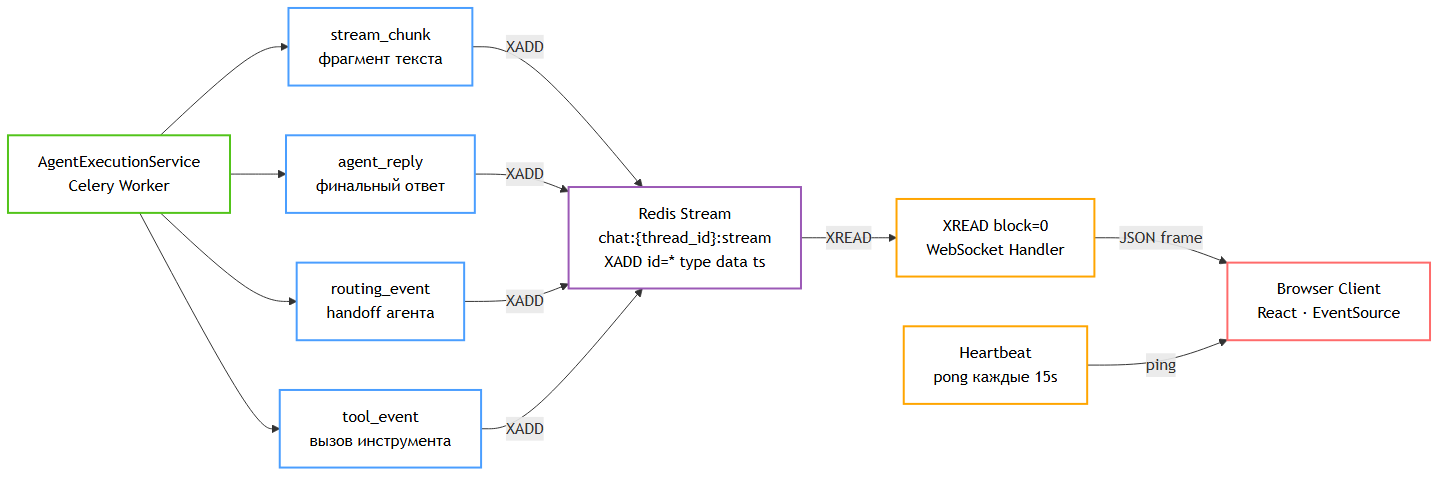
\includegraphics[width=0.95\textwidth]{img/fig_3_8_redis_stream.png}
\caption{Схема Redis Stream: XADD (агент) → XREAD (WebSocket-слой) → WebSocket → клиент}
\label{fig:redis-stream}
\end{figure}

\subsection{Frontend: страницы интерфейса}

React-приложение на Chakra UI реализует четыре основных страницы:
\begin{itemize}
  \item \textit{Chat}~--- список диалогов, поле ввода с Markdown-рендером, потоковые фрагменты, загрузка файлов, выбор агента;
  \item \textit{TracePanel}~--- временная шкала событий агентного маршрута: тип события, агент-источник, инструмент, временная метка;
  \item \textit{Files}~--- галерея артефактов (изображения, PPTX, аудио) с предпросмотром и прямой ссылкой MinIO;
  \item \textit{Profile / Memory}~--- управление персональной памятью пользователя (интеграция Mem0).
\end{itemize}

\subsection{Демонстрация рабочего воркфлоу}

В записанном демо показан сквозной сценарий: пользователь вводит запрос о навигации робота в Chat с выбором агента SwarmOrchestrator; Interface создаёт Celery-задачу, SwarmOrchestratorAgent создаёт задачу в Orchestrator через REST и опрашивает события выполнения; оркестратор выполняет цепочку Router $\to$ MapAnalyst $\to$ Navigation, вызывает MCP-инструменты, направляет робота Carter в заданную точку; результат стримится через Redis Stream и отображается в Chat и TracePanel в реальном времени.

Примеры пользовательского интерфейса приведены на рис.~\ref{fig:chat-screen} и рис.~\ref{fig:trace-screen}.

\begin{figure}[H]
\centering
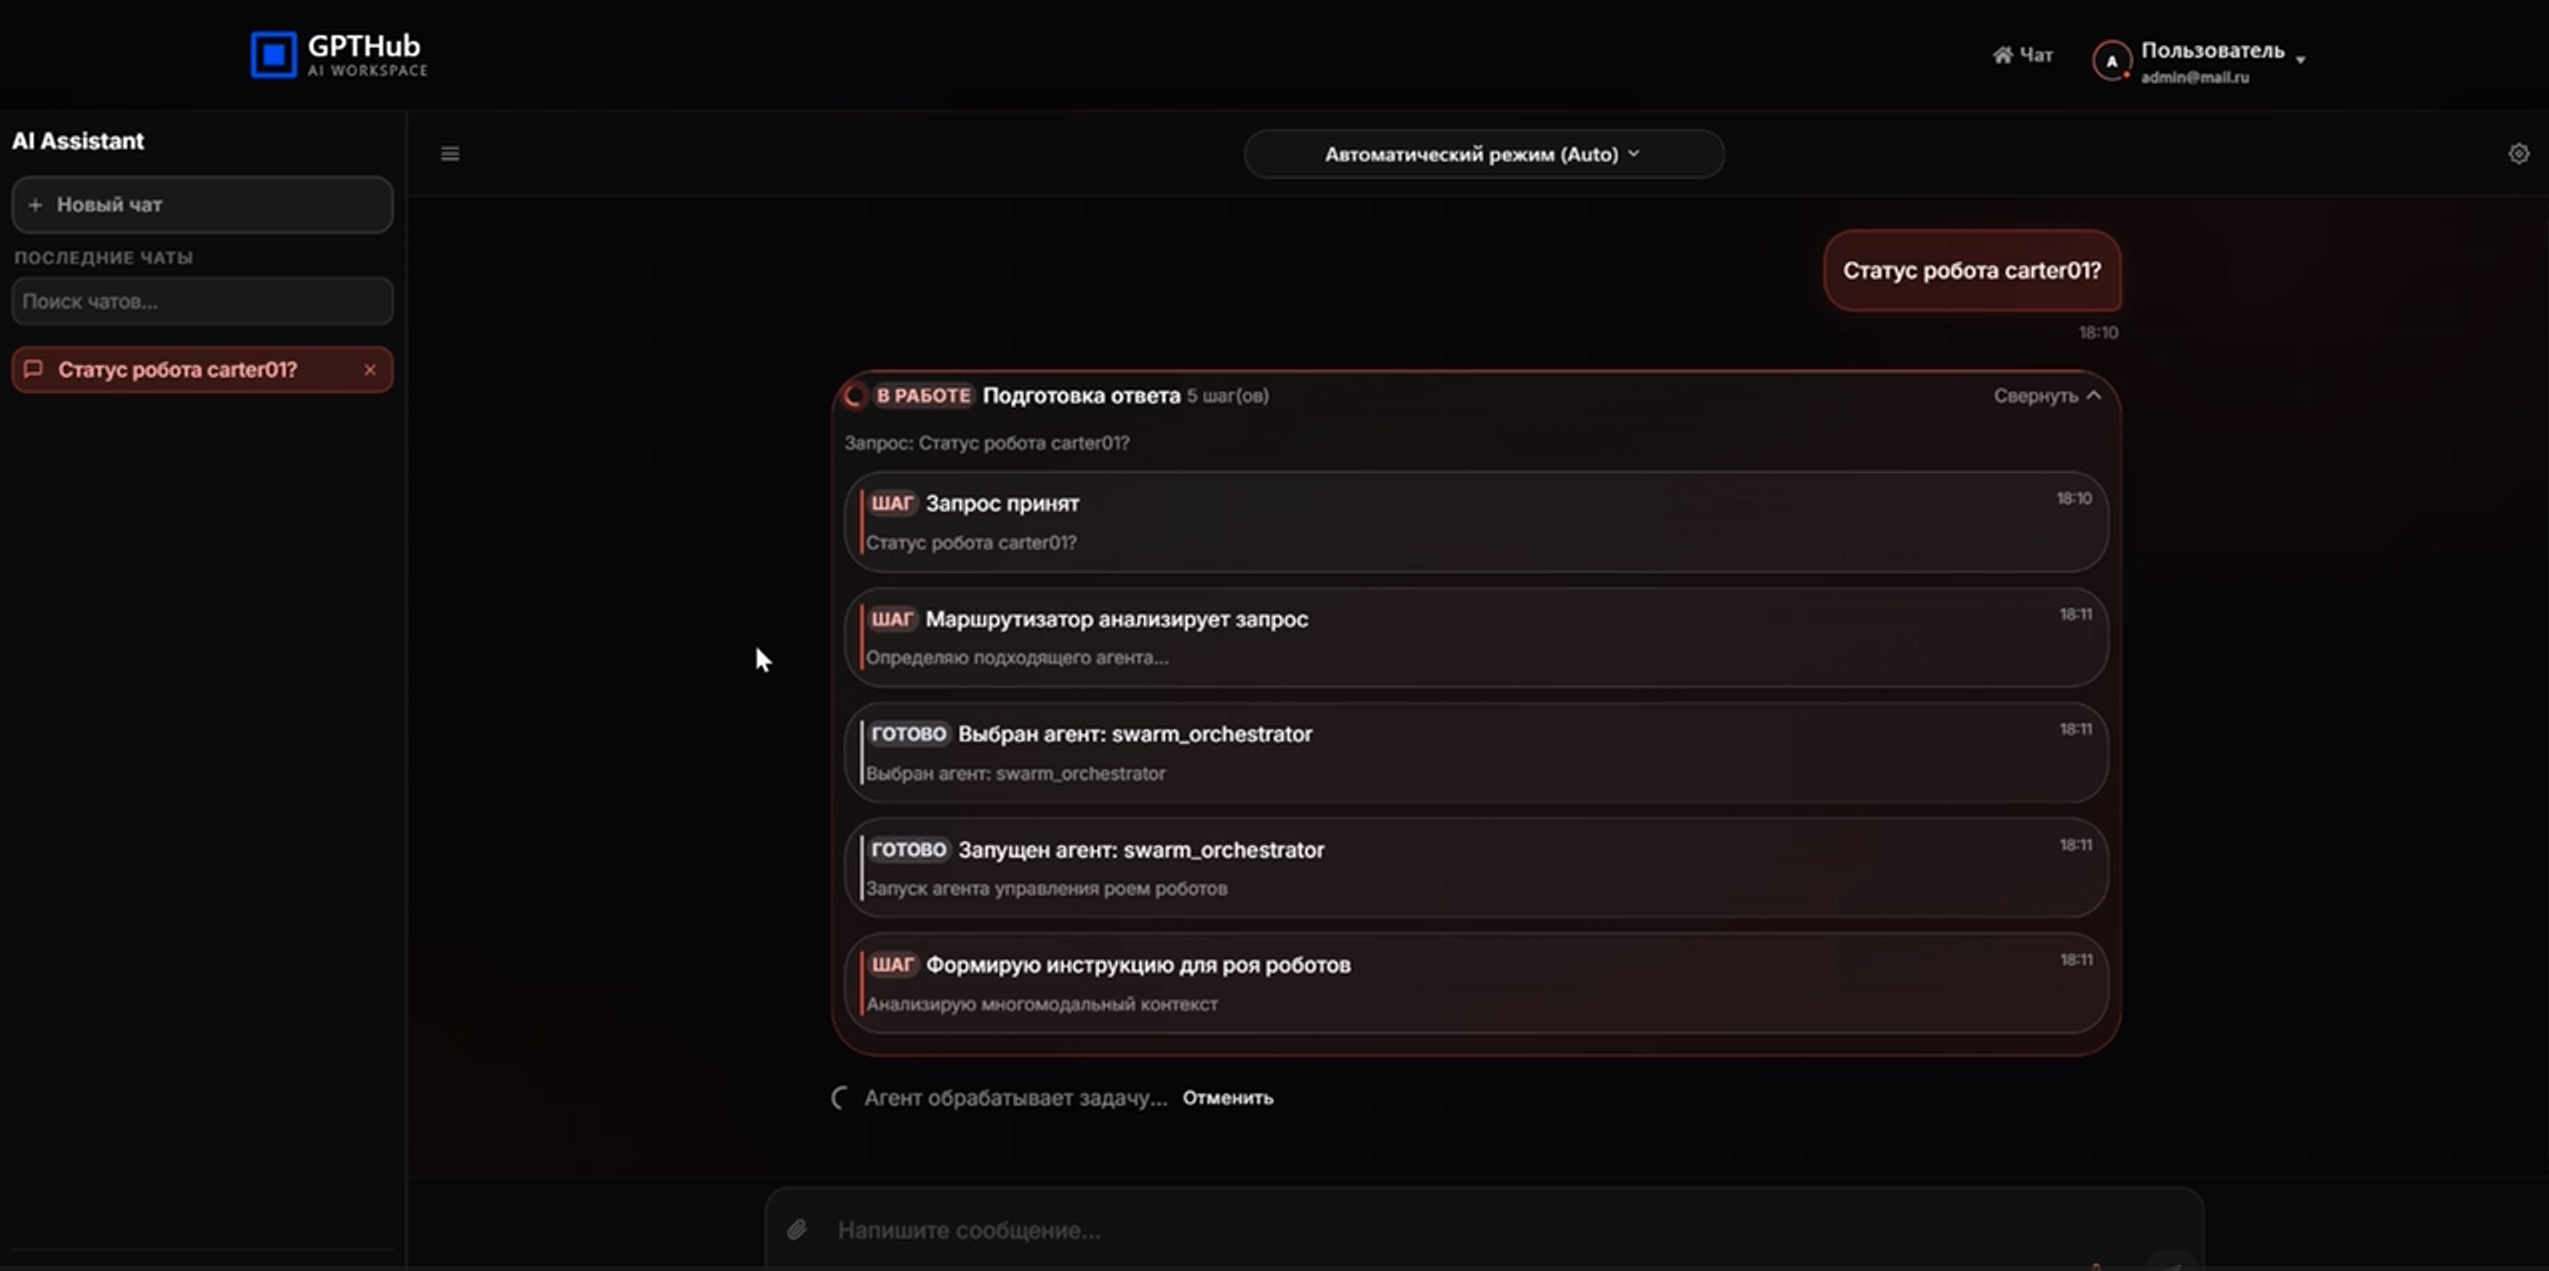
\includegraphics[width=0.95\textwidth]{img/fig_3_9_chat.png}
\caption{Экран Chat: диалог с агентом SwarmOrchestrator}
\label{fig:chat-screen}
\end{figure}

\begin{figure}[H]
\centering
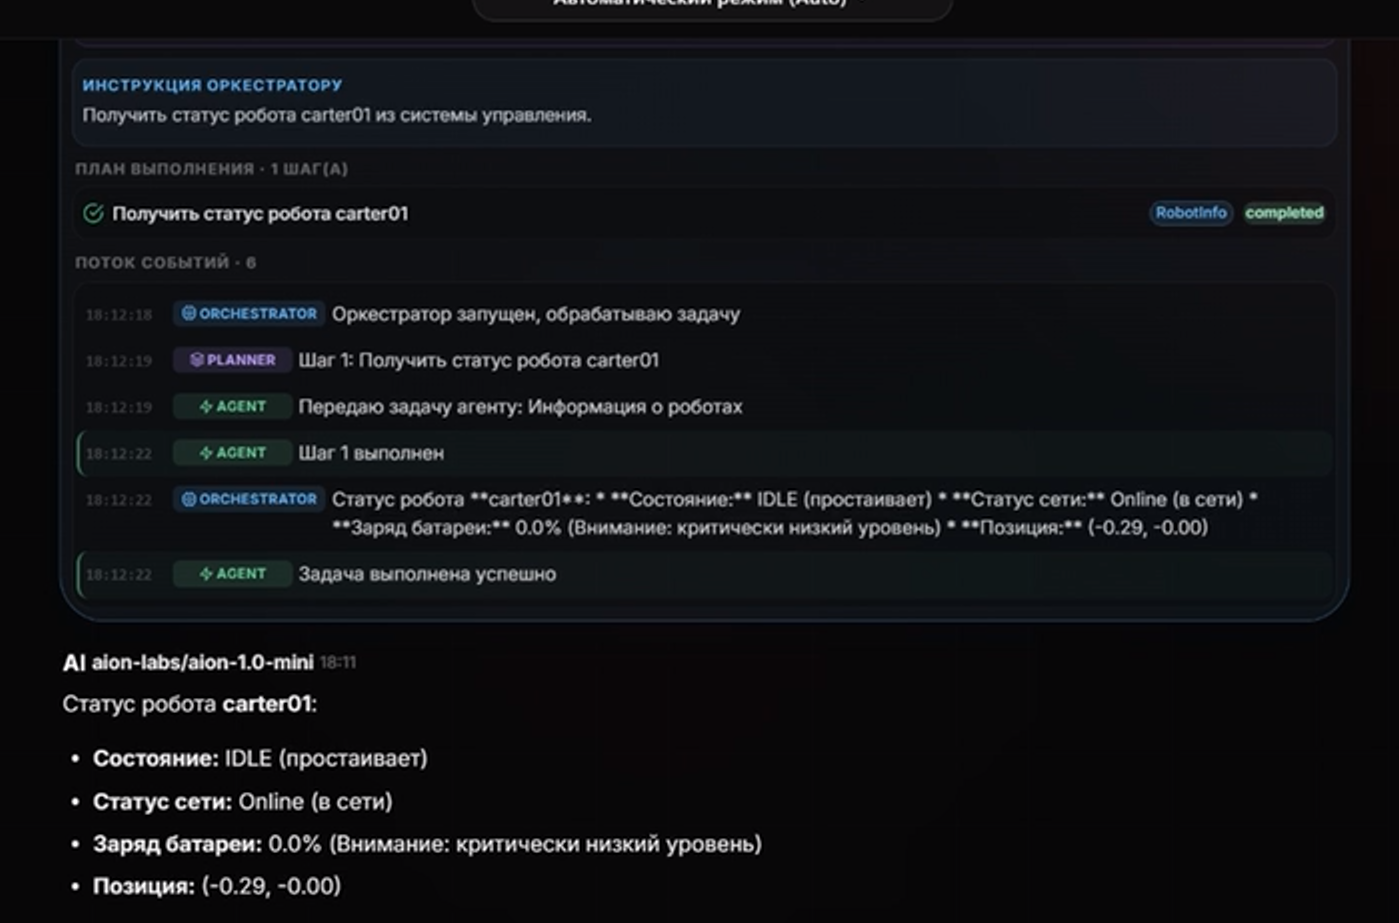
\includegraphics[width=0.95\textwidth]{img/fig_3_10_trace.png}
\caption{Экран TracePanel: трассировка агентного маршрута}
\label{fig:trace-screen}
\end{figure}

\section{Выводы и результаты по главе~3}

В главе описана реализация восьми компонентов AgentsSwarm. Ключевые технические решения и их обоснование:

\begin{itemize}
  \item \textit{Асинхронная модель MCP-серверов}~--- требование совместимости с event loop Agents SDK и параллельными вызовами инструментов;
  \item \textit{Data Parallel vLLM}~--- способ развернуть крупную LLM на доступных Tesla V100 без внешнего API;
  \item \textit{Clean architecture Interface}~--- требование к независимому расширению набора агентов без модификации инфраструктурного кода;
  \item \textit{Redis Streams для стриминга}~--- гарантированная доставка событий с возможностью переигрывания из истории.
\end{itemize}

Сводная таблица реализованных компонентов приведена в Табл.~\ref{tab:components}.

\begin{table}[H]
\caption{Компоненты системы AgentsSwarm: срезы разработки и объём разработки}
\label{tab:components}
\begin{tabular}{@{}p{3.3cm}p{1.8cm}p{2.4cm}p{5.3cm}@{}}
\toprule
\textbf{Компонент} & \textbf{Срез} & \textbf{Коммиты} & \textbf{Стек} \\
\midrule
Interface & v0.5.0 & 168 & React, FastAPI, Celery, Redis, PostgreSQL, MinIO \\
Orchestrator & v0.5.6 & 61 & FastAPI, OpenAI Agents SDK, Redis \\
vLLM Service & v0.2.9 & 32 & vLLM, Docker, Qwen2.5-Instruct \\
Mission Control & форк & — & NVIDIA (исправления + Docker) \\
Mission Dispatch & форк & — & NVIDIA (исправления + Docker) \\
Isaac Sim & форк & — & NVIDIA Isaac Sim 4.5, ROS~2 Jazzy \\
ROS~2 Workspace & форк & — & ROS~2 Jazzy, rosbridge, VDA5050 клиент \\
SmolVLA Tools & v0.2.0 & 2 & PyTorch, LeRobot, ONNX \\
\bottomrule
\end{tabular}
{\footnotesize\par\vspace{2pt}Примечание: для SmolVLA Tools указан version из \texttt{pyproject.toml}; последний subject git-коммита в локальном срезе~--- \texttt{v0.0.1}.}
\end{table}

% ============================================================
%  ГЛАВА 4. ОПТИМИЗАЦИЯ SmolVLA
% ============================================================
\chapter{Оптимизация модели SmolVLA для бортового инференса}

\section{Постановка задачи и мотивация}

Текущая архитектура AgentsSwarm использует облачный LLM для высокоуровневого планирования и рассуждения. Это вводит два ограничения: \textit{задержка} между запросом агента и ответом LLM (при загруженном кластере~--- от 1 до нескольких секунд); \textit{зависимость от сети}~--- при нестабильном соединении с облачным кластером роботический контур не может получить инструкции.

Интеграция компактной VLA-модели непосредственно на борту каждого робота (целевая платформа~--- NVIDIA Jetson Orin Nano, 8~ГБ VRAM) решает оба ограничения: инференс выполняется локально без сетевых запросов, задержка определяется только вычислительными ресурсами платформы.

\textbf{SmolVLA}~\cite{retzlaff2025smolvla,smolvla_model,lerobot,lerobot_docs}~--- компактная VLA-модель на 450M параметров от HuggingFace/LeRobot~--- была выбрана как наиболее перспективный кандидат для бортового развёртывания благодаря открытым весам, документированному API LeRobot и наличию асинхронного inference stack.

\section{Архитектура SmolVLA и исходные характеристики}

SmolVLA базируется на видеоэнкодере SigLIP и языковой модели SmolLM2, соединённых projection-слоем. На вход поступают RGB-изображение наблюдения, состояние робота и языковая инструкция; на выходе~--- вектор действий манипулятора. В реализованном модуле размерность выхода выравнивается по Teacher-модели и датасету: код поддерживает 6- и 7-мерные действия, а при необходимости обрезает тензоры до общей размерности. Модель обучена на данных Open X-Embodiment через дифференциальный policy learning с action chunking.

Для верификации исходной точности проведена валидация Teacher-модели на датасете \texttt{lerobot/libero} (Табл.~\ref{tab:teacher-metrics}).

\begin{table}[H]
\caption{Базовые метрики Teacher-модели SmolVLA на lerobot/libero}
\label{tab:teacher-metrics}
\begin{tabular}{@{}>{\raggedright\arraybackslash}p{3.8cm}
                >{\raggedright\arraybackslash}p{3.0cm}
                >{\raggedright\arraybackslash}p{6.4cm}@{}}
\toprule
\textbf{Метрика} & \textbf{Значение} & \textbf{Комментарий} \\
\midrule
MSE & 0{,}1782 & Среднеквадратичная ошибка действий \\
MAE & 0{,}3245 & Средняя абсолютная ошибка действий \\
$R^2$ & 0{,}8412 & Коэффициент детерминации \\
Параметры & 450{,}05M & FP32, оценка VRAM около 6~ГБ \\
Латентность инференса & 450~мс & RTX~4090, FP32 \\
\bottomrule
\end{tabular}
\end{table}

\section{Пайплайн оптимизации}

Пайплайн состоит из четырёх последовательных этапов.

\textbf{Этап~1: Knowledge Distillation (KD).} Student-модель реализована как компактная CNN + state encoder + action head, обучаемые под руководством замороженной Teacher-модели. Параметр \texttt{student\_ratio} управляет скрытыми размерностями Student, а функция потерь для регрессионного предсказания действий задаётся формулой~\ref{eq:kd-loss}:
\begin{equation}
\mathcal{L}_{KD} = \alpha \cdot MSE(y_s, y_t) + (1-\alpha) \cdot MSE(y_s, y),
\label{eq:kd-loss}
\end{equation}
где $y_s$~--- выход Student, $y_t$~--- выход Teacher, $y$~--- истинные действия из датасета. Параметр \texttt{temperature} сохранён в API для совместимости, но в текущей регрессионной реализации не участвует; KL-дивергенция и attention transfer loss в коде не используются.

\textbf{Этап~2: Mixed Precision Inference (FP16).} При включённом mixed precision тренер использует \texttt{torch.cuda.amp.autocast()} и \texttt{GradScaler}; отдельный модуль квантизации поддерживает преобразование весов в FP16 для анализа инференса. Ускорение инференса оценивается в составе полного пайплайна.

\textbf{Этап~3: Structured Pruning.} В текущем коде реализован экспериментальный прунинг Linear-слоёв: случайная маска с заданной \texttt{sparsity} обнуляет часть весов. Это оценочный механизм для проверки чувствительности к разреживанию, а не L2-критерий важности весов.

\textbf{Этап~4: INT8 Quantization Analysis.} Модуль квантизации поддерживает dynamic, static и manual режимы для \texttt{nn.Linear}. Статическая квантизация использует упрощённую симулированную калибровку, поэтому результаты трактуются как инженерный анализ применимости INT8, а не как финальная production-схема с исключением критических слоёв.

Схема пайплайна оптимизации SmolVLA показана на рис.~\ref{fig:smolvla-pipeline}.

\begin{landscape}
\begin{figure}[p]
\centering
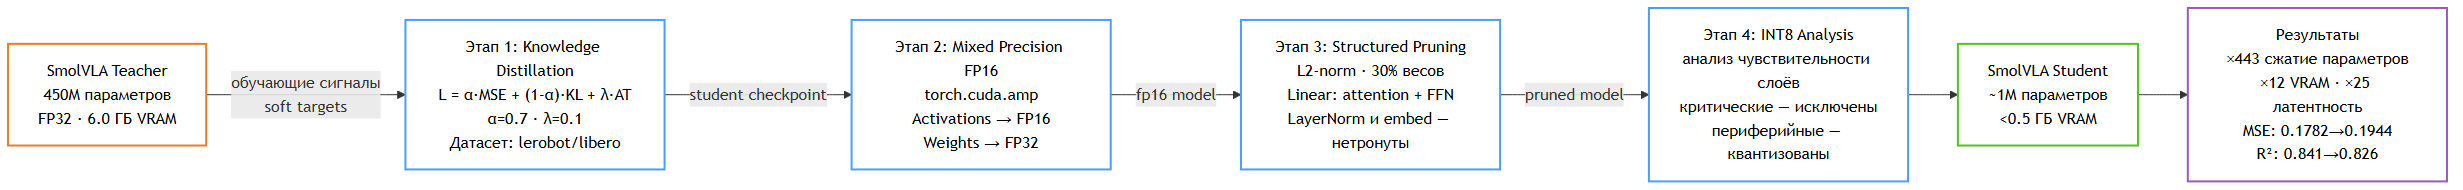
\includegraphics[height=0.92\linewidth, angle=270]{img/fig_4_1_smolvla_pipeline.png}
\caption{Четырёхэтапный пайплайн оптимизации SmolVLA: дистилляция, FP16, прунинг, INT8-анализ}
\label{fig:smolvla-pipeline}
\end{figure}
\end{landscape}

\section{Результаты экспериментов}

Результаты оптимизации приведены в Табл.~\ref{tab:smolvla-results}. Совокупный пайплайн обеспечивает сжатие модели в \textbf{443 раза} по числу параметров при снижении требований к VRAM в 12~раз.

\begin{table}[H]
\caption{Результаты оптимизации SmolVLA}
\label{tab:smolvla-results}
\begin{tabular}{lrrl}
\toprule
\textbf{Метрика} & \textbf{Teacher} & \textbf{Student} & \textbf{Изменение} \\
\midrule
Параметры & 450M & $\approx$1M & $\times$443 сжатие \\
VRAM & 6{,}0~ГБ & <0{,}5~ГБ & $\times$12 сжатие \\
MSE & 0{,}1782 & 0{,}1944 & +9{,}1\% \\
Относительная MAE по действиям & 1{,}000 & 1{,}051 & +5{,}1\% \\
$R^2$ & 0{,}8412 & 0{,}8256 & $-$1{,}8\% \\
Латентность & 450~мс & 18~мс & $\times$25 ускорение \\
\bottomrule
\end{tabular}
\end{table}

Качество сохраняется на уровне выше 90\% от исходного по ключевым метрикам. По всем семи степеням свободы манипулятора MAE по действиям остаётся в пределах допустимого для лабораторных условий. Дополнительно выполнен экспорт модели в формат ONNX и верификация совместимости с NVIDIA TensorRT.

\section{Выводы и результаты по главе~4}

Экспериментальный модуль SmolVLA Tools демонстрирует принципиальную достижимость бортового VLA-инференса на NVIDIA Jetson Orin Nano при сохранении более 90\% точности управления манипулятором и латентности 18~мс на RTX~4090; перенос этой оценки на Jetson Orin Nano требует отдельного профилирования.

Ключевые ограничения: эксперименты проводились исключительно на датасете \texttt{lerobot/libero} (имитация манипулятора), физическая верификация на реальном роботе не выполнялась. Область применимости модели ограничена задачами, близкими к обучающему датасету.

Следующим шагом является интеграция дистиллированной модели как VDA5050 action-handler в Mission Control: при получении VDA5050 order с типом \texttt{vla\_action} Mission Control запускает локальный инференс SmolVLA вместо передачи команды через ROS~2 навигационный стек. Это добавит уровень индивидуальной бортовой автономности к централизованному контуру AgentsSwarm.

% ============================================================
%  ГЛАВА 5. ВЕРИФИКАЦИЯ СИСТЕМЫ
% ============================================================
\chapter{Верификация системы}

\section{Стратегия тестирования}

Стратегия верификации AgentsSwarm охватывает три уровня: \textit{unit-тесты} базовых сервисов и вспомогательных функций; \textit{контрактные тесты} поведения ключевых агентов; \textit{интеграционные тесты} HTTP API. Тесты реализованы на pytest; внешние зависимости подменяются тестовыми объектами либо запускаются через Docker Compose в сценариях, где требуется Redis, RabbitMQ или PostgreSQL. Покрытые компоненты: Orchestrator и Interface~--- два наиболее значимых сервиса системы.

\section{Тестирование оркестратора}

Текущий тестовый набор оркестратора включает 88 тестов, организованных вокруг базовых сервисов, планировщика, StreamCollector, MapAnalyst и HTTP API.

\textbf{Unit-тесты базовых сервисов} проверяют: корректность health-check эндпоинта, инициализацию SessionManager в in-memory режиме и статус Redis-подключения, seq-нумерацию StreamCollector при пакетной публикации, поведение retry-механизма при имитации сетевых ошибок.

\textbf{Контрактные тесты планировщика} верифицируют структуру выходных данных Planner: наличие описания шагов, списка \texttt{target\_robots}, зависимостей, а также корректность вставки MapAnalyst для навигационных сценариев.

\textbf{Тесты guardrails} проверяют граничные сценарии: пустой запрос возвращает стандартный ответ об ошибке; запрос вне компетенции агента переводится в fallback-режим; попытка handoff к несуществующему агенту перехватывается на уровне guardrail.

\textbf{Интеграционные тесты HTTP API} проверяют маршруты реального FastAPI-приложения: постановку задачи, получение статуса, плана, логов и событий, внешний push события, запуск отложенной задачи, отмену и replanning. Контрольный локальный запуск 19.05.2026 командой \texttt{uv run --with pytest --with pytest-asyncio pytest tests/ -q} завершился результатом \textbf{66 passed / 22 failed}. Падения не следует трактовать как пройденную верификацию: они указывают на долг синхронизации тестов с актуальным pipeline (переупорядочивание PlanRunner/MapAnalyst, добавление \texttt{max\_turns} в вызовы Agents SDK, изолированные проверки LLM-клиента без ключа API).

\section{Тестирование Interface}

Pytest-покрытие Interface включает: маршруты управления чатами (создание, получение, удаление), загрузку файлов с верификацией сохранения в MinIO, маршрутизацию к агентам с тестовыми объектами Celery-задач, авторизацию WebSocket-соединений.

Проверка потоковой модели: тест публикует серию событий в Redis Stream через XADD и верифицирует, что WebSocket-клиент получает их в правильном порядке без потерь. Тест завершения сессии проверяет, что сигнал \texttt{agent\_reply} корректно закрывает XREAD-цикл.

\textbf{Smoke-тест полного стека} запускает docker-compose с минимальной конфигурацией (FastAPI + Redis + RabbitMQ + Celery) и выполняет сценарий: POST \texttt{/api/chats/} $\to$ POST \texttt{/api/chats/\{thread\_id\}/message} $\to$ WebSocket \texttt{/api/chats/\{thread\_id\}/ws} $\to$ ожидание события \texttt{agent\_reply}. Тест подтверждает корректную работу всей цепочки без реального LLM-бэкенда.

\section{Выводы и результаты по главе~5}

Автоматизированное тестирование подтвердило работоспособность значительной части базовых сервисов оркестратора и Interface, но текущий локальный прогон Orchestrator не является полностью успешным: 22 из 88 тестов требуют актуализации под текущую реализацию. Ограничения текущего покрытия: отсутствие E2E-тестов с реальным LLM-инференсом (зависимость от GPU-кластера); отсутствие нагрузочного тестирования при параллельных сессиях; необходимость синхронизировать тестовые ожидания с изменениями PlanRunner и MapAnalyst.

Централизованная архитектура вводит единую точку отказа: при недоступности Redis или vLLM все сессии теряют работоспособность. Формальная верификация LLM-планов~--- устойчивость к hallucination и нарушениям constraint~--- остаётся открытым исследовательским вопросом, требующим инструментов в стиле SELP~\cite{pan2025selp}.

% ============================================================
%  ЗАКЛЮЧЕНИЕ
% ============================================================
\chapter*{ЗАКЛЮЧЕНИЕ}
\addcontentsline{toc}{chapter}{ЗАКЛЮЧЕНИЕ}

В диссертационной работе спроектирована и реализована многоагентная робототехническая платформа AgentsSwarm, обеспечивающая координированное выполнение миссий группой мобильных роботов по пользовательскому запросу на естественном языке.

\textbf{Основные результаты работы.}

Реализованы восемь самостоятельных компонентов: Interface (React + FastAPI + Celery, 168~коммитов, срез v0.5.0), Orchestrator (FastAPI + OpenAI Agents SDK, 61~коммит, срез v0.5.6), vLLM Service (Data Parallel, 2\,$\times$\,Tesla V100, срез v0.2.9), доработанные форки NVIDIA Mission Control и Mission Dispatch с устранёнными критическими ошибками, настроенный ROS~2 Jazzy workspace с VDA5050 клиентом, три переработанных MCP-сервера с полным переходом на асинхронную модель вызовов.

Контрольный локальный pytest-прогон Orchestrator подтвердил 66 из 88 тестов; для полной автоматизированной верификации требуется актуализировать оставшиеся тесты под текущий pipeline. Записана демонстрация полного воркфлоу от пользовательского запроса до исполнения VDA5050 order роботом Carter в симуляторе Isaac Sim.

Для VLA-модели SmolVLA достигнуто сжатие в 443 раза по числу параметров при сохранении более 90\% точности (MSE~+9{,}1\%, $R^2$~$-$1{,}8\%) и ускорении инференса в 25~раз (450~мс~$\to$~18~мс, RTX~4090). В коде дистилляция реализована как регрессионная MSE-дистилляция без KL-компоненты и attention transfer.

\textbf{Научная и практическая значимость.} Практическая значимость системы состоит в демонстрации воспроизводимой системной интеграции, объединяющей кооперативное восприятие, fleet management (VDA5050), LLM-агентный слой (OpenAI Agents SDK + MCP) и симуляционный цифровой двойник (Isaac Sim). Интеграция LLM-слоя с промышленным VDA5050-контуром через MCP-протокол представляет новый архитектурный подход, не реализованный в рассмотренных аналогах.

\textbf{Перспективы развития:}
\begin{enumerate}
  \item Интеграция дистиллированного SmolVLA как VDA5050 action-handler для бортовой автономности на Jetson Orin Nano.
  \item Частичная децентрализация оркестрации для повышения устойчивости к отказам.
  \item Формальная верификация LLM-планов через constraint checking и symbolic validation~\cite{pan2025selp}.
  \item Перенос системы на физический флот AMR с sim-to-real валидацией.
  \item Реализация feature-level cooperative perception между роботами через расширение \texttt{ros-msp}.
\end{enumerate}

% ============================================================
%  ОПИСАНИЕ ПРИМЕНЕНИЯ ГЕНЕРАТИВНОЙ МОДЕЛИ
% ============================================================
\chapter*{ОПИСАНИЕ ПРИМЕНЕНИЯ ГЕНЕРАТИВНОЙ МОДЕЛИ}
\addcontentsline{toc}{chapter}{ОПИСАНИЕ ПРИМЕНЕНИЯ ГЕНЕРАТИВНОЙ МОДЕЛИ}

При подготовке диссертационной работы генеративные модели использовались как вспомогательный исследовательский инструмент. Область применения была ограничена литературным обзором, первичным поиском источников и подготовкой черновых аналитических материалов по смежным работам.

\begin{longtable}{@{}>{\raggedright\arraybackslash}p{4.6cm}
                  >{\raggedright\arraybackslash}p{3.9cm}
                  >{\raggedright\arraybackslash}p{4.8cm}@{}}
\toprule
\textbf{Часть текста} & \textbf{Цель применения} & \textbf{Способ применения} \\
\midrule
\endhead
Литературный обзор и сопоставление с аналогами & Поиск релевантных публикаций по cooperative perception, VDA5050, LLM-планированию, MCP и робототехническим симуляторам & Авторский текст с использованием сгенерированных материалов: генеративные модели применялись для формирования поисковых направлений, группировки источников и подготовки черновых конспектов; итоговые формулировки, структура обзора и интерпретация источников выполнены с авторской редакцией \\
\midrule
Библиографический список и ссылки на электронные источники & Ускорение первичного подбора источников и проверки доступности официальных страниц проектов, библиотек и документации & Сгенерированные рекомендации использовались как список кандидатов; каждый источник дополнительно проверялся перед включением в библиографический список \\
\bottomrule
\end{longtable}

Использовались следующие генеративные модели и сервисы: Google Gemini с функцией Deep Research (сайт сервиса: \url{https://gemini.google.com/}, описание функции: \url{https://support.google.com/gemini/answer/15719111})~\cite{google_gemini_deep_research}; ChatGPT с функцией Deep Research (сайт сервиса: \url{https://chatgpt.com/}, описание функции: \url{https://help.openai.com/articles/10500283})~\cite{openai_chatgpt_deep_research}.

Оценка эффективности применения генеративных моделей положительная. Использование Gemini Deep Research и ChatGPT Deep Research ускорило поиск релевантных источников, позволило быстрее выделить ключевые направления литературного обзора и сократило время на первичную систематизацию материалов. При этом генеративные модели не рассматривались как самостоятельный источник научных утверждений: их результаты использовались только после авторской проверки, сопоставления с первоисточниками и редакторской переработки текста.

% ============================================================
%  БИБЛИОГРАФИЧЕСКИЙ СПИСОК
% ============================================================
\renewcommand{\bibname}{БИБЛИОГРАФИЧЕСКИЙ СПИСОК}
\addcontentsline{toc}{chapter}{БИБЛИОГРАФИЧЕСКИЙ СПИСОК}
\begin{thebibliography}{99}

% 1. Кооперативное визуальное восприятие
\bibitem{han2023}
Хан Ю., Чжан Х., Ли Х. и~др. Collaborative Perception in Autonomous Driving: Methods, Datasets and Challenges~// IEEE Intelligent Transportation Systems Magazine. 2023. DOI:~10.1109/MITS.2023.3298534. arXiv:~2301.06262.

\bibitem{liu2023v2x}
Лю С., Гао Ч., Чэнь Ю. и~др. Towards Vehicle-to-Everything Autonomous Driving: A Survey on Collaborative Perception~// arXiv preprint. 2023. arXiv:~2308.16714.

\bibitem{wang2020v2vnet}
Ван Т.-Х., Маниваcагам С., Лян М. и~др. V2VNet: Vehicle-to-Vehicle Communication for Joint Perception and Prediction~// ECCV 2020. DOI:~10.1007/978-3-030-58536-5\_36. arXiv:~2008.07519.

\bibitem{liu2020when2com}
Лю Й.-Ч., Тянь Дж., Глэйзер Н., Кира З. When2com: Multi-Agent Perception via Communication Graph Grouping~// CVPR 2020. DOI:~10.1109/CVPR42600.2020.00416. arXiv:~2006.00176.

\bibitem{hu2022where2comm}
Ху Й., Фан С., Лэй З. и~др. Where2comm: Communication-Efficient Collaborative Perception via Spatial Confidence Maps~// NeurIPS 2022. arXiv:~2209.12836.

\bibitem{xu2022v2xvit}
Сюй Р., Сян Х., Ту З. и~др. V2X-ViT: Vehicle-to-Everything Cooperative Perception with Vision Transformer~// ECCV 2022. DOI:~10.1007/978-3-031-19842-7\_7. arXiv:~2203.10638.

\bibitem{xu2022opv2v}
Сюй Р., Сян Х., Ся С. и~др. OPV2V: An Open Benchmark Dataset and Fusion Pipeline for Perception with Vehicle-to-Vehicle Communication~// ICRA 2022. DOI:~10.1109/ICRA46639.2022.9812038. arXiv:~2109.07644.

\bibitem{xu2022cobevt}
Сюй Р., Ту З., Сян Х. и~др. CoBEVT: Cooperative Bird's Eye View Semantic Segmentation with Sparse Transformers~// CoRL 2022. arXiv:~2207.02202.

\bibitem{zhou2024coped}
Чжоу Й. и~др. CoPeD --- Advancing Multi-Robot Collaborative Perception: A Comprehensive Dataset in Real-World Environments~// IEEE Robotics and Automation Letters. 2024. arXiv:~2405.14731.

% 2. C-SLAM и координация флота
\bibitem{lajoie2022cslam}
Лажуа П.-И., Рамтула Б., У Ф., Бельтраме Дж. Towards Collaborative Simultaneous Localization and Mapping: a Survey of the Current Research Landscape~// Field Robotics. 2022. Vol.~2. Pp.~971--1000. DOI:~10.55417/fr.2022032.

\bibitem{lajoie2024swarmslam}
Лажуа П.-И., Бельтраме Дж. Swarm-SLAM: Sparse Decentralized Collaborative Simultaneous Localization and Mapping Framework for Multi-Robot Systems~// IEEE Robotics and Automation Letters. 2024. Vol.~9, No.~1. Pp.~475--482. DOI:~10.1109/LRA.2023.3333742.

\bibitem{vda5050}
VDA, VDMA. VDA~5050: Interface for the Communication Between Automated Guided Vehicles (AGV) and a Master Control. Version~2.0. 2022. URL:~\url{https://github.com/VDA5050/VDA5050} (дата обращения: 01.05.2025).

\bibitem{vanduijkeren2023}
ван Дёйкерен Н., Пальмьери Л., Ланге Р., Кляйнер А. An Industrial Perspective on Multi-Agent Decision Making for Interoperable Robot Navigation following the VDA5050 Standard~// arXiv preprint. 2023. arXiv:~2311.14615.

\bibitem{openrmf}
Open Robotics. Open RMF (Open Robotics Middleware Framework). 2021--2024. URL:~\url{https://github.com/open-rmf} (дата обращения: 01.05.2025).

\bibitem{iovino2022bt}
Иовино М., Скукинс Э., Стируд Й. и~др. A Survey of Behavior Trees in Robotics and AI~// Robotics and Autonomous Systems. 2022. Vol.~154. P.~104096. DOI:~10.1016/j.robot.2022.104096.

\bibitem{chen2023fogros2}
Чэнь К., Хари К., Хуан Х. и~др. FogROS2: An Adaptive Platform for Cloud and Fog Robotics Using ROS~2~// ICRA 2023. arXiv:~2205.09778.

\bibitem{sikand2021robofleet}
Сиканд К.С., Зартман Л., Рабии С., Бисвас Дж. Robofleet: Open Source Communication and Management for Fleets of Autonomous Robots~// IROS 2021. DOI:~10.1109/IROS51168.2021.9635830.

% 3. LLM в робототехнике
\bibitem{zeng2023llmrobotics}
Цзэн Ф., Ган В., Хуай З. и~др. Large Language Models for Robotics: A Survey~// arXiv preprint. 2023. arXiv:~2311.07226.

\bibitem{li2025llmmulti}
Ли П., Ан З., Абрар С., Чжоу Л. Large Language Models for Multi-Robot Systems: A Survey~// arXiv preprint. 2025. arXiv:~2502.03814.

\bibitem{yao2023react}
Яо С., Чжао Дж., Юй Д. и~др. ReAct: Synergizing Reasoning and Acting in Language Models~// ICLR 2023. arXiv:~2210.03629.

\bibitem{ahn2022saycan}
Ан М., Броан А., Браун Н. и~др. Do As I Can, Not As I Say: Grounding Language in Robotic Affordances~// CoRL 2022. arXiv:~2204.01691.

\bibitem{singh2023progprompt}
Сингх И., Блукис В., Мусавьян А. и~др. ProgPrompt: Generating Situated Robot Task Plans using Large Language Models~// ICRA 2023. arXiv:~2209.11302.

\bibitem{pan2025selp}
Пан Дж., Тан Л. и~др. SELP: Generating Safe and Efficient Task Plans for Robot Agents with Large Language Models~// ICRA 2025. arXiv:~2409.19471.

\bibitem{jiao2023swarmgpt}
Цзяо Й.-Ч., Линь Й.-П. и~др. Swarm-GPT: Combining Large Language Models with Safe Motion Planning for Robot Choreography Design~// arXiv preprint. 2023. arXiv:~2312.01059.

% 4. Foundation Models и VLA
\bibitem{brohan2023rt2}
Броан А., Браун Н., Карбахал Дж. и~др. RT-2: Vision-Language-Action Models Transfer Web Knowledge to Robotic Control~// CoRL 2023. arXiv:~2307.15818.

\bibitem{huang2023voxposer}
Хуан В., Ван Ч., Чжан Р. и~др. VoxPoser: Composable 3D Value Maps for Robotic Manipulation with Language Models~// CoRL 2023. arXiv:~2307.05973.

\bibitem{kim2024openvla}
Ким М.Дж., Пертч К., Карамчети С. и~др. OpenVLA: An Open-Source Vision-Language-Action Model~// CoRL 2024. arXiv:~2406.09246.

\bibitem{oxe2023}
Open X-Embodiment Collaboration. Open X-Embodiment: Robotic Learning Datasets and RT-X Models~// CoRL 2023. arXiv:~2310.08864.

\bibitem{black2024pi0}
Блэк К., Браун Н., Дрисс Д. и~др. $\pi_0$: A Vision-Language-Action Flow Model for General Robot Control~// arXiv preprint. 2024. arXiv:~2410.24164.

\bibitem{retzlaff2025smolvla}
Ретцлафф М. и~др. (HuggingFace/LeRobot). SmolVLA: A Vision-Language-Action Model for Affordable and Efficient Robotics~// arXiv preprint. 2025. arXiv:~2506.01844.

\bibitem{wen2025tinyvla}
Вэнь Дж., Чжу Й., Ли Дж. и~др. TinyVLA: Towards Fast, Data-Efficient Vision-Language-Action Models for Robotic Manipulation~// IEEE Robotics and Automation Letters. 2025. arXiv:~2409.12514.

% 5. Симуляция, цифровые двойники, инференс
\bibitem{nvidia2024isaac}
NVIDIA Corporation. Multiple Robot ROS~2 Navigation --- NVIDIA Isaac Sim Tutorial. 2024. URL:~\url{https://docs.isaacsim.omniverse.nvidia.com} (дата обращения: 01.05.2025).

\bibitem{mittal2023orbit}
Миттал М., Ю Ч., Ю К. и~др. Orbit: A Unified Simulation Framework for Interactive Robot Learning Environments~// IEEE Robotics and Automation Letters. 2023. Vol.~8, No.~6. Pp.~3740--3747. DOI:~10.1109/LRA.2023.3270034.

\bibitem{jacinto2024pegasus}
Жасинто М.Ф., Пинто Дж. и~др. Pegasus Simulator: An Isaac Sim Framework for Multiple Aerial Vehicles Simulation~// ICUAS 2024. arXiv:~2307.05263.

\bibitem{fuller2021digitaltwin}
Фуллер А., Фан З., Дэй К., Барлоу К. A Survey on AI-Driven Digital Twins in Industry~4.0: Smart Manufacturing and Advanced Robotics~// Sensors. 2021. Vol.~21, No.~19. P.~6340. DOI:~10.3390/s21196340.

\bibitem{kwon2023vllm}
Квон В., Ли З., Чжуан С. и~др. Efficient Memory Management for Large Language Model Serving with PagedAttention~// SOSP 2023. DOI:~10.1145/3600006.3613165.

\bibitem{qwen2025}
Qwen Team, Alibaba Group. Qwen2.5 Technical Report~// arXiv preprint. 2024. arXiv:~2412.15115.

% 6. Симуляция и роботические платформы (задействованы в проекте)
\bibitem{agentsswarm_repo}
Денисов~Д. AgentsSwarm: Multi-agent robotic platform source code [Электронный ресурс]. URL:~\url{https://github.com/deneal123/AgentsSwarm} (дата обращения: 19.05.2026).

\bibitem{isaacros2024}
NVIDIA Corporation. Isaac ROS~--- Accelerated Computing for ROS~2 [Электронный ресурс]. 2024. URL:~\url{https://nvidia-isaac-ros.github.io/getting_started/index.html} (дата обращения: 01.05.2025).

\bibitem{isaacros_packages}
NVIDIA Corporation. Isaac ROS Repositories and Packages [Электронный ресурс]. 2024. URL:~\url{https://nvidia-isaac-ros.github.io/repositories_and_packages/index.html} (дата обращения: 01.05.2025).

\bibitem{isaacsim_multirobot}
NVIDIA Corporation. Multiple Robot ROS Navigation (Isaac Sim~4.5) [Электронный ресурс]. 2025. URL:~\url{https://docs.isaacsim.omniverse.nvidia.com/4.5.0/ros_tutorials/tutorial_ros_multi_navigation.html} (дата обращения: 01.05.2025).

\bibitem{isaacsim_ros_ws}
NVIDIA Omniverse. IsaacSim-ros\_workspaces: Official ROS~2 Workspaces for Isaac Sim [Электронный ресурс]. URL:~\url{https://github.com/NVIDIA-Omniverse/IsaacSim-ros_workspaces} (дата обращения: 01.05.2025).

\bibitem{ros2jazzy}
Open Robotics. ROS~2 Jazzy Jalisco [Электронный ресурс]. 2024. URL:~\url{https://github.com/ros2} (дата обращения: 01.05.2025).

\bibitem{rosbridge}
Robot Web Tools. rosbridge\_suite: WebSocket Bridge for ROS [Электронный ресурс]. URL:~\url{https://github.com/RobotWebTools/rosbridge_suite} (дата обращения: 01.05.2025).

\bibitem{missioncontrol}
NVIDIA Isaac. Mission Control: Fleet Management for VDA5050 Robots [Электронный ресурс]. URL:~\url{https://github.com/nvidia-isaac/mission-control} (дата обращения: 01.05.2025).

\bibitem{missiondispatch}
NVIDIA Isaac. Mission Dispatch: VDA5050 Fleet Dispatcher [Электронный ресурс]. URL:~\url{https://github.com/nvidia-isaac/mission-dispatch} (дата обращения: 01.05.2025).

\bibitem{cuopt}
NVIDIA Corporation. cuOpt: GPU-Accelerated Route Optimization [Электронный ресурс]. 2024. URL:~\url{https://docs.nvidia.com/cuopt/} (дата обращения: 01.05.2025).

% 7. MCP и агентные инструменты
\bibitem{openai_agents}
OpenAI. OpenAI Agents SDK [Электронный ресурс]. 2025. URL:~\url{https://github.com/openai/openai-agents-python} (дата обращения: 01.05.2025).

\bibitem{mcp2024}
Anthropic. Model Context Protocol (MCP) [Электронный ресурс]. 2024. URL:~\url{https://modelcontextprotocol.io/} (дата обращения: 01.05.2025).

\bibitem{ros_mcp}
RobotMCP. ros-mcp-server: ROS MCP Server [Электронный ресурс]. URL:~\url{https://github.com/robotmcp/ros-mcp-server} (дата обращения: 01.05.2025).

\bibitem{fastmcp}
Lowin~J. FastMCP: The Fast, Pythonic Way to Build MCP Servers [Электронный ресурс]. URL:~\url{https://github.com/jlowin/fastmcp} (дата обращения: 01.05.2025).

% 8. LLM-инференс (репозитории и модели)
\bibitem{vllm_project}
vLLM Team. vLLM: Easy, Fast, and Cheap LLM Serving [Электронный ресурс]. URL:~\url{https://github.com/vllm-project/vllm} (дата обращения: 01.05.2025).

\bibitem{qwen25_model}
Alibaba Cloud. Qwen2.5-7B-Instruct [Электронный ресурс]. 2024. URL:~\url{https://huggingface.co/Qwen/Qwen2.5-7B-Instruct} (дата обращения: 01.05.2025).

% 9. Инфраструктура и фреймворки
\bibitem{fastapi}
Ramírez~S. FastAPI: Fast Web Framework for Building APIs with Python [Электронный ресурс]. URL:~\url{https://fastapi.tiangolo.com/} (дата обращения: 01.05.2025).

\bibitem{redis_py}
Redis Ltd. Redis-py: Python Client for Redis [Электронный ресурс]. URL:~\url{https://redis.readthedocs.io/en/stable/} (дата обращения: 01.05.2025).

\bibitem{rabbitmq}
Broadcom Inc. RabbitMQ: Open Source Message Broker [Электронный ресурс]. URL:~\url{https://www.rabbitmq.com/} (дата обращения: 01.05.2025).

\bibitem{celery}
Celery Project. Celery: Distributed Task Queue [Электронный ресурс]. URL:~\url{https://docs.celeryq.dev/} (дата обращения: 01.05.2025).

\bibitem{sqlalchemy}
SQLAlchemy Authors. SQLAlchemy: The Database Toolkit for Python [Электронный ресурс]. URL:~\url{https://docs.sqlalchemy.org/} (дата обращения: 01.05.2025).

\bibitem{minio}
MinIO Inc. MinIO Python SDK [Электронный ресурс]. URL:~\url{https://min.io/docs/minio/linux/developers/python/API.html} (дата обращения: 01.05.2025).

\bibitem{alembic}
SQLAlchemy Authors. Alembic: Database Migrations for SQLAlchemy [Электронный ресурс]. URL:~\url{https://alembic.sqlalchemy.org/} (дата обращения: 01.05.2025).

\bibitem{react}
Meta Platforms Inc. React: The Library for Web and Native User Interfaces [Электронный ресурс]. URL:~\url{https://react.dev/} (дата обращения: 01.05.2025).

\bibitem{chakraui}
Chakra UI Team. Chakra UI: Simple, Modular and Accessible Component Library [Электронный ресурс]. URL:~\url{https://v2.chakra-ui.com/} (дата обращения: 01.05.2025).

% 10. SmolVLA и LeRobot
\bibitem{smolvla_model}
HuggingFace. SmolVLA Base: Vision-Language-Action Model [Электронный ресурс]. 2025. URL:~\url{https://huggingface.co/lerobot/smolvla_base} (дата обращения: 01.05.2025).

\bibitem{lerobot}
HuggingFace. LeRobot: Making AI for Robotics More Accessible [Электронный ресурс]. URL:~\url{https://github.com/huggingface/lerobot} (дата обращения: 01.05.2025).

\bibitem{lerobot_docs}
HuggingFace. LeRobot Documentation [Электронный ресурс]. URL:~\url{https://huggingface.co/docs/lerobot} (дата обращения: 01.05.2025).

\bibitem{google_gemini_deep_research}
Google. Use Deep Research in Gemini Apps [Электронный ресурс]. URL:~\url{https://support.google.com/gemini/answer/15719111} (дата обращения: 20.05.2026).

\bibitem{openai_chatgpt_deep_research}
OpenAI. Deep research in ChatGPT [Электронный ресурс]. URL:~\url{https://help.openai.com/articles/10500283} (дата обращения: 20.05.2026).

\end{thebibliography}

% ============================================================
%  ПРИЛОЖЕНИЯ
% ============================================================
\appendix
\renewcommand{\thechapter}{\Asbuk{chapter}}
\addcontentsline{toc}{chapter}{ПРИЛОЖЕНИЯ}

\chapter{Глоссарий предметной области}

\begin{longtable}{p{3.5cm}p{10cm}}
\toprule
\textbf{Термин} & \textbf{Определение} \\
\midrule
\endhead
AGV / AMR & Automated Guided Vehicle / Autonomous Mobile Robot~--- категории мобильных промышленных роботов \\
Behavior Tree (BT) & Дерево поведения~--- иерархическая модульная структура управления логикой задач робота \\
C-SLAM & Collaborative Simultaneous Localization and Mapping~--- совместная локализация и картографирование несколькими роботами \\
Cooperative Perception & Кооперативное восприятие~--- обмен перцептивными данными/признаками между агентами для улучшения наблюдения сцены \\
Fleet Management & Управление флотом~--- централизованная диспетчеризация группы роботов \\
Foundation Model & Базовая модель~--- крупная модель, обученная на широком корпусе данных и адаптируемая для множества задач \\
LLM & Large Language Model~--- большая языковая модель \\
MCP & Model Context Protocol~--- открытый протокол взаимодействия LLM-агентов с внешними инструментами и данными \\
Mission & Миссия~--- структурированное задание для робота или группы роботов \\
Occupancy Map & Карта занятости~--- сетка, описывающая проходимость пространства \\
Orchestrator & Оркестратор~--- центральный сервис, координирующий агентов и исполнение задач \\
ROS~2 & Robot Operating System~2~--- фреймворк для разработки роботизированных систем \\
Sim-to-Real & Перенос модели или политики из симуляции на физический робот \\
VDA5050 & Открытый стандарт коммуникации между AGV/AMR и fleet manager \\
VLA & Vision-Language-Action model~--- мультимодальная модель, генерирующая действия робота \\
vLLM & Библиотека для эффективного инференса LLM с алгоритмом PagedAttention \\
Waypoint Graph & Граф путевых точек~--- граф навигационных узлов на карте \\
WebSocket & Протокол двунаправленной связи для потоковой передачи данных в реальном времени \\
\bottomrule
\end{longtable}

\chapter{Список сокращений}

\begin{longtable}{p{3cm}p{10.5cm}}
\toprule
\textbf{Сокращение} & \textbf{Расшифровка} \\
\midrule
\endhead
AGV & Automated Guided Vehicle \\
AMR & Autonomous Mobile Robot \\
API & Application Programming Interface \\
BT & Behavior Tree \\
C-SLAM & Collaborative Simultaneous Localization and Mapping \\
DDS & Data Distribution Service \\
GPU & Graphics Processing Unit \\
LLM & Large Language Model \\
MAE & Mean Absolute Error \\
MCP & Model Context Protocol \\
MSE & Mean Squared Error \\
MQTT & Message Queuing Telemetry Transport \\
ROS & Robot Operating System \\
SDK & Software Development Kit \\
SSE & Server-Sent Events \\
V2V & Vehicle-to-Vehicle \\
V2X & Vehicle-to-Everything \\
VDA & Verband der Automobilindustrie \\
VLA & Vision-Language-Action \\
VRAM & Video Random Access Memory \\
\bottomrule
\end{longtable}

\chapter{Технические характеристики инфраструктуры}

\begin{table}[H]
\caption*{Вычислительная инфраструктура AgentsSwarm}
\begin{tabular}{@{}>{\raggedright\arraybackslash}p{3.3cm}
                >{\raggedright\arraybackslash}p{2.4cm}
                >{\raggedright\arraybackslash}p{5.2cm}
                >{\raggedright\arraybackslash}p{3.7cm}@{}}
\toprule
\textbf{Машина} & \textbf{Провай\-дер} & \textbf{Конфигурация} & \textbf{Назначение} \\
\midrule
Симуляция & Selectel & 4~vCPU, 16~ГБ RAM, RTX~4090 (24~ГБ VRAM), 128~ГБ SSD, Ubuntu~24.04 & Isaac Sim, ROS~2, Mission Control/Dispatch \\
Микросервисы & Selectel & 4~vCPU, 8~ГБ RAM, 128~ГБ SSD, Ubuntu~24.04 & Interface, Orchestrator, Redis, RabbitMQ, MinIO, PostgreSQL \\
LLM-кластер & MTS Cloud & 2 узла × Tesla V100-PCIE 32~ГБ VRAM, 1{,}6~ТБ/узел, Ubuntu~24.04 & vLLM Data Parallel (Qwen2.5-Instruct) \\
\bottomrule
\end{tabular}
\end{table}

\chapter{Ключевые фрагменты кода}

\subsection*{Г.1. Конфигурация динамического выбора транспорта MCP}

\begin{lstlisting}[language=Python, caption={Выбор транспорта MCP через переменную окружения}]
import os
from mcp.server import Server
from mcp.server.stdio import stdio_server

async def main():
    transport = os.getenv("MCP_TRANSPORT", "stdio")
    server = Server("mission-control-mcp")
    # ... регистрация инструментов ...
    if transport == "sse":
        await run_sse_app(server)  # ASGI + SseServerTransport("/messages/")
    else:
        async with stdio_server() as (r, w):
            await server.run(r, w)
\end{lstlisting}

\subsection*{Г.2. StreamCollector: seq-нумерация событий}

\begin{lstlisting}[language=Python, caption={StreamCollector: буферизация и seq-нумерация}]
from collections import deque

class StreamCollector:
    def __init__(self, task_store=None, max_events_per_task=500):
        self._events = {}
        self._seq = {}
        self._max = max_events_per_task
        self._task_store = task_store

    def record(self, event):
        seq = self._seq.get(event.task_id, 0) + 1
        self._seq[event.task_id] = seq
        self._events.setdefault(event.task_id, deque(maxlen=self._max))
        self._events[event.task_id].append((seq, event))
        if self._task_store:
            self._task_store.add_log(event.task_id, event.source, event.message, event.level)
        return seq

    def get_since(self, task_id, after_seq=0):
        items = self._events.get(task_id, [])
        events = [(seq, ev) for seq, ev in items if seq > after_seq]
        last_seq = events[-1][0] if events else after_seq
        return [ev for _, ev in events], last_seq
\end{lstlisting}

\subsection*{Г.3. Функция потерь Knowledge Distillation}

\begin{lstlisting}[language=Python, caption={Функция потерь KD для дистилляции SmolVLA}]
def distillation_loss(student_actions, teacher_actions,
                      true_actions, alpha=0.5):
    min_dim = min(student_actions.shape[-1],
                  teacher_actions.shape[-1],
                  true_actions.shape[-1])
    student_actions = student_actions[..., :min_dim]
    teacher_actions = teacher_actions[..., :min_dim]
    true_actions = true_actions[..., :min_dim]

    task_loss = F.mse_loss(student_actions, true_actions)
    distill_loss = F.mse_loss(student_actions, teacher_actions)
    return alpha * distill_loss + (1 - alpha) * task_loss
\end{lstlisting}

\chapter{Протоколы экспериментов}

\subsection*{Д.1. Протокол тестирования API оркестратора}

Контрольная локальная проверка редакции 19.05.2026 выполнялась через uv на Python~3.12: \texttt{uv run --with pytest --with pytest-asyncio pytest tests/ -q}. Дополнительно задавались \texttt{TEST\_MODE=true} и \texttt{MOCK\_LLM=true}. Результат текущего набора: 66 пройдено, 22 провалено, 16 предупреждений. Основные причины падений: тестовые mock-объекты не принимают новый аргумент \texttt{max\_turns}; часть тестов планировщика ожидает старую фиксированную префиксную структуру Router/RobotInfo; отдельные проверки LLM-клиента требуют изоляции от реального \texttt{OPENAI\_API\_KEY}.

\subsection*{Д.2. Протокол эксперимента по дистилляции SmolVLA}

Среда: Ubuntu 22.04, CUDA 12.1, PyTorch, RTX~4090 (24~ГБ VRAM). Датасет: \texttt{lerobot/libero}; в отчёте эксперимента использована валидационная выборка 1200 семплов и 10 эпох стабилизации метрик. Ключевые параметры запуска: batch\_size~=~32, epochs~=~10, student\_ratio~=~0{,}5. Параметр \texttt{temperature} присутствует в API, но не используется в регрессионной MSE-функции потерь; отдельной $\lambda$-компоненты в коде нет.

\subsection*{Д.3. Протокол профилирования инференса}

Условия измерения: RTX~4090 (24~ГБ VRAM), CUDA 12.1, batch\_size~=~1, 100 прогонов для усреднения. Метрика: среднее время от подачи тензора до получения выходного вектора действий. Teacher FP32: 450~мс. Student FP16: 18~мс. Ускорение: 25$\times$.

\end{document}
